\documentclass[12pt]{article}
\usepackage[utf8]{inputenc}
\usepackage{hyperref}
\usepackage{listings}
\usepackage{color}
\definecolor{dkgreen}{rgb}{0,0.6,0}
\definecolor{gray}{rgb}{0.5,0.5,0.5}
\definecolor{mauve}{rgb}{0.58,0,0.82}
\lstset{frame=tb,
  language=python,
  aboveskip=3mm,
  belowskip=3mm,
  showstringspaces=false,
  columns=flexible,
  basicstyle={\small\ttfamily},
  numbers=none,
  numberstyle=\tiny\color{gray},
  keywordstyle=\color{blue},
  commentstyle=\color{dkgreen},
  stringstyle=\color{mauve},
  breaklines=true,
  breakatwhitespace=true,
  tabsize=3
}
\usepackage{tcolorbox}%forbox
\usepackage{amsmath} %for math
\usepackage{blindtext} %not important. used to write lorem epsim.... thingy. not required
\usepackage{hyperref} %used to link contents to content menu
\usepackage{multicol} % used to split page into multiple columns
\usepackage{fontspec} % font 
% Inserting times new roman
\setmainfont[ 
BoldFont=timesbd.ttf,
ItalicFont=timesi.ttf,
BoldItalicFont=timesbi.ttf
]{times.ttf}
\usepackage{graphicx} %used to include images
\graphicspath{ {figures/} }
\usepackage{array}
\usepackage{geometry} % to customize page styles
 \geometry{
 a4paper,
 total={170mm,257mm},
 left=25.4mm,
 right=26.4mm,
 top=25.4mm,
 bottom=25.4mm
 }
 
\begin{document} %document starts from here
\pagenumbering{gobble} %used to give blank page number. try to do this in word hahaha
\begin{center} % content to center
    \textbf{\begin{huge} % Search for different types of fonts in latex to know more
    SEMINAR REPORT ON\\
    \end{huge}}
   \vspace{10mm} %used to give vertical space ie.,Next line will be 10mm from the above line in this case
    
    \begin{Large}\textbf{
    CONVOLUTIONAL NEURAL NETWORKS FOR  \vspace{3mm}\\COMPUTER VISION}
    \end{Large} %textbf{} used to make the charectr inside the bracket bold
    
    \vspace{7mm}
    
    \textbf{\textit{\begin{large}A seminar report submitted in partial fulfillment for the award of the degree of\end{large}}}
    
    \vspace{5mm}
    
    \begin{Large}\textbf{
    BACHELOR OF TECHNOLOGY}
    \end{Large}
    
    \vspace{5mm}
    
    \begin{Large}\textbf{
    \textit{IN}}
    \end{Large}
    
    \vspace{7mm}
    
    \begin{Large}\textbf{
    ELECTRONICS \& COMMUNICATION ENGINEERING}
    \end{Large}
    \vspace{18mm}
    
    \textbf{\textit{\begin{large}Submitted by\end{large}}} % Here to make the font bold and italic, \textbf{\textit{content}} is used
    
    \vspace{7mm}
    
    \textbf{\begin{huge}
    SUJITH S
    \end{huge}\begin{huge}
    (14402113)
    \end{huge}}
    
    \vspace{10mm}
    
    \begin{figure}[h]
    \centering
    
\includegraphics[width=0.55\textwidth]{sct.jpg} %to include pic.
    \end{figure}
    
    \vspace{15mm}
    
    \begin{large}\textbf{
    DEPT. OF ELECTRONICS\&COMMUNICATION ENGINEERING\\SREE CHITRA THIRUNAL COLLEGE OF ENGINEERING,\\THIRUVANANTHAPURAM-18\\ \vspace{4mm} SEPTEMBER 2017}
    \end{large}
    
    
\end{center}
\newpage
\pagenumbering{gobble}
\begin{center}
\begin{large}
 \textbf{SREE CHITRA THIRUNAL COLLEGE OF ENGINEERING}
 \vspace{5mm}
\end{large}
\begin{Large}

 \textbf{THIRUVANANTHAPURAM-18}
\end{Large}
\begin{figure}[h]
    \centering
    
\includegraphics[width=0.55\textwidth]{sct.jpg}
    
\end{figure}
\begin{LARGE}

\textbf{CERTIFICATE}\\
\end{LARGE}
 \end{center}
 \par This is to certify that this seminar entitled “\textbf{Convolutional Neural Networks For Computer Vision}" is a bonafide record of the seminar done by  SUJITH S in partial fulfilment of the requirements for the award of Bachelor of Technology degree in Electronics and Communication Engineering under the University of Kerala,   during the  academic year 2017-18\\
 \\ \\ \\ \textbf{SEMINAR COORDINATORS: \hspace{55mm} SEMINAR GUIDE\\ \vspace{6mm}}

\begin{center}
\begin{multicols}{3}

    
\textbf{\small Smt. ASHA S}
\vspace{2mm}\\Assistant Professor

Department of ECE

SCTCE

\columnbreak %Column break point

\textbf{\small Sri. GEORGE M JOSEPH}
\vspace{2mm}\\Associate professor

Department of ECE 

SCTCE


\columnbreak

\textbf{\small Smt. ASHA S}
\vspace{2mm}\\Associate professor

Department of ECE

SCTCE

\end{multicols}
\vspace{20mm}

\textbf{\large HEAD OF DEPARTMENT}
\vspace{2mm}\\
\textbf{\small Prof. Dr. Sheeja M K}

Professor

Department of ECE

SCT College of Engineering
\end{center}
\newpage
\pagenumbering{roman}
.
\vspace{25mm}
\begin{center}
\section*{\fontsize{16}{18}\selectfont Acknowledgement}
\end{center}
\vspace{10mm}
\par  I take this opportunity to express my profound gratitude and deep regards to our seminar coordinators Mrs. Asha S (Asst.Professor of Dept. Of ECE, SCTCE) and Mr. George M Joseph for their exemplary guidance, monitoring and constant encouragement throughout the course of this seminar. The help and guidance given by them from time to time shall carry me in a long way in the journey of life in which i am about to embark.\\

\par I also take this opportunity to express a deep sense of gratitude to Prof. Dr. S H Anilkumar (Principal, SCTCE), for his cordial support, valuable information and guidance, which helped us in completing this project through various stages.\\

\par I am really thankful to Dr. Sheeja M K (Head of department, ECE, SCTCE) for her invaluable guidance and assistance, without which the accomplishment of the task would have been impossible.\\

\par I would not forget to remember Mrs. Preetha V H (Assistant professor, ECE Department, SCTCE) and Mr. Kumar G S (Assistant professor, ECE Department, SCTCE) for their encouragement and more over for their timely support and guidance till completion of this seminar.\\

\par I am also obliged to staff members of SCTCE for the valuable information provided by them in their respective fields. We are grateful for their co-operation during the period of our assignment.\\

\par Lastly, I thank my parents, brothers, sisters and friends for their constant encouragement without which this assignment would have been impossible.\\
\vspace{10mm}
\begin{flushright}
\textbf{SUJITH S}
\end{flushright}

\addcontentsline{toc}{section}{Acknowledgement}
\newpage
.
\vspace{50mm}
\begin{center}
\section*{\fontsize{16}{18}\selectfont Abstract}
\end{center}
\par This seminar report is based on the seminar held during the academic year 2017-18. The report focuses convolutional neural networks and computer vision allowing the reader to understand the underlying concept of CNN and also an introduction to neural networks. After giving a brief introduction to Neural networks, We discuss about some machine learning processes to give a basic understanding of the concept of convolutional neural networks. 
\vspace{5mm}
\par The second section focuses entirely on convolutional neural networks and the different layers in it. The third section is about the recent developments in convolutional neural networks in the field of computer vision and object detection and the final session is about the practical side and implementation of convolutional neural network.
\addcontentsline{toc}{section}{Abstract}

\newpage
\pagenumbering{gobble}
\tableofcontents
\newpage
\pagenumbering{gobble}

\listoffigures
\listoftables
\newpage

.
\vspace{15mm} 
\pagenumbering{arabic}
\section{\fontsize{14}{14}\selectfont Introduction}
 \par This report is to give the readers an introduction to convolutional neural networks and computer vision.  Convolutional neural network is a type of Artificial neural network used specifically for object detection. It can also be used for speech recognition.It Sounds like a combination of biology and math with a little CS, but these networks have been some of the most influential innovations in the field of computer vision. 2012 was the first year that neural nets grew to prominence as Alex Krizhevsky used them to win that year’s ImageNet competition (basically, the annual Olympics of computer vision), dropping the classification error record from 26\% to 15\%, an astounding improvement at the time.Ever since then, a host of companies have been using deep learning at the core of their services. Facebook uses neural nets for their automatic tagging algorithms, Google for their photo search, Amazon for their product recommendations, Pinterest for their home feed personalization, and Instagram for their search infrastructure. Basically, it is one of the growing and most innovative field in deep learning and computer vision. The companies that have lots of data are the ones that have an inherent advantage over the rest of the competition. The more training data that you can give to a network, the more training iterations you can make, the more weight updates you can make, and the better tuned to the network is when it goes to production. Facebook (and Instagram) can use all the photos of the billion users it currently has, Pinterest can use information of the 50 billion pins that are on its site, Google can use search data, and Amazon can use data from the millions of products that are bought every day and this is how big companies use convolutional neural networks. Now for a beginning, this report will give the basics introduction to convolutional neural networks and at the end of this, the readers will be able to implement it.
\section{\fontsize{14}{14}\selectfont Human brain}
\par The struggle to understand the brain has been made easier because of the pioneering work of Ramón y Cajál (1911), who introduced the idea of neurons as structural constituents of the brain. Typically, neurons are five to six orders of magnitude slower than silicon logic gates; events in a silicon chip happen in the nanosecond range, whereas neural events happen in the millisecond range. However, the brain makes up for the relatively slow rate of operation of a neuron by having a truly staggering number of neurons (nerve cells) with massive interconnections between them. It is estimated that there are approximately 10 billion neurons in the human cortex, and 60 trillion synapses or connections (Shepherd and Koch, 1990). The net result is that the brain is an enormously efficient structure. Specifically, the energetic efficiency
of the brain is approximately $10^{16}$ joules (J) per operation per second, whereas the corresponding value for the best computers is orders of magnitude larger. 

The brain is a highly complex, nonlinear, and parallel computer
(information-processing system). It has the capability to organize its structural constituents, known as neurons, so as to perform certain computations (e.g., pattern recognition, perception, and motor control) many times faster than the fastest digital computer in existence today. Consider, for example, human vision, which is an information-processing task. It is the function of the visual system to provide a representation of the environment around us and, more important, to supply the information we need to interact with the environment. To be specific, the brain routinely accomplishes perceptual recognition tasks (e.g., recognizing a familiar face embedded in an unfamiliar scene) in approximately 100–200 ms, whereas tasks of much lesser complexity take a great deal longer on a powerful computer.


\begin{figure}[h]
    \centering
    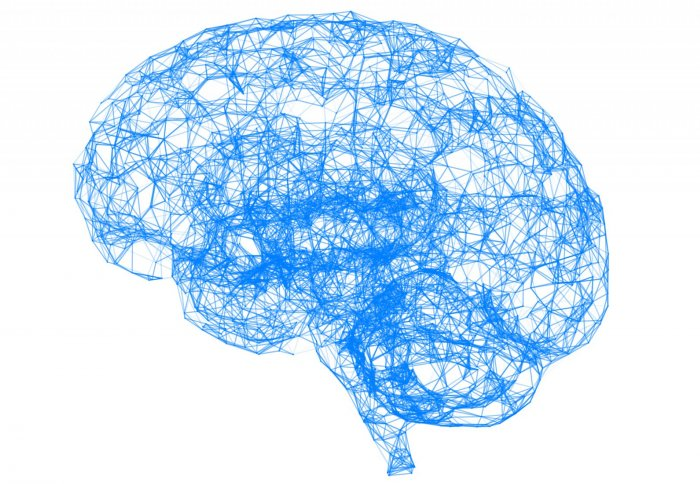
\includegraphics[width=0.25 \textwidth]{brain.jpg}
    \caption{Human brain}
    \label{fig:mesh1}
    Representation of human brain with neural networks 
\end{figure}

For another example, consider the sonar of a bat. Sonar is an active echolocation system. In addition to providing information about how far away a target (e.g., a flying insect) is, bat sonar conveys information about the relative velocity of the target, the size of the target, the size of various features of the target, and the azimuth and elevation of the target. The complex neural computations needed to extract all this information from the target echo occur within a brain the size of a plum. Indeed, an echo-locating bat can pursue and capture its target with a facility and success rate that would be the envy of a radar or sonar engineer. 

How, then, does a human brain or the brain of a bat do it? At birth, a brain already has considerable structure and the ability to build up its own rules of behavior through what we usually refer to as “experience.” Indeed, experience is built up over time, with much of the development (i.e., hardwiring) of the human brain taking place during the first two years from birth, but the development continues well beyond that stage.



\section{\fontsize{14}{14}\selectfont Artificial neural network}
\par Artificial  Neural  Networks  (ANNs)  are  relatively  crude  electronic  models based  on  the  neural  structure  of  the brain.  The  brain  learns  from  experience. Artificial neural networks try to mimic the functioning of brain. Even simple animal brains   are   capable   of   functions   that   are currently   impossible   for   computers. Computers  do  the  things  well,  but  they  have  trouble recognizing  even  simple patterns.  

\begin{figure}[h]
	\centering
    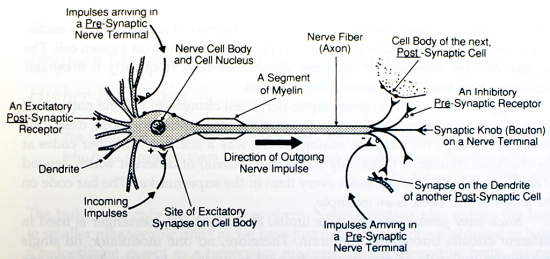
\includegraphics[width=0.55 \textwidth]{b.png}
    \caption{Neuron}
    \label{fig:mesh2}
    A single biological neuron(Nerve)
     
\end{figure}

As a matter of fact, classical artificial intelligence concentrated, based on this hypothesis,on symbolic forms of representing knowledge and in particular on propositional and predicated
logic. (Artificial) neural networks, on the other hand, are no physical symbol systems, since they do not process symbols, but rather much more elementary signals, which, taken individually, rarely have a (clear) meaning. As a consequence (artificial) neural networks are often called “sub-symbolic.” However, if the ability to process symbols is necessary to produce intelligent behavior, then it is unnecessary to study (artificial) neural networks in artificial intelligence. \vspace{10mm}
    \subsection{Introduction to artificial neural networks}

	Artificial neural networks (ANNs) or connectionist systems are computing systems inspired by the biological neural networks that constitute animal brains. Such systems learn (progressively improve performance) to do tasks by considering examples, generally without task-specific programming. For example, in image recognition, they might learn to identify images that contain cats by analyzing example images that have been manually labeled as "cat" or "no cat" and using the results to identify cats in other images. They have found most use in applications difficult to express in a traditional computer algorithm using rule-based programming.Warren McCulloch and Walter Pitts (1943) created a computational model for neural networks based on mathematics and algorithms called threshold logic. This model paved the way for neural network research to split into two approaches. One approach focused on biological processes in the brain while the other focused on the application of neural networks to artificial intelligence. This work led to work on nerve networks and their link to finite automata.
	
	 \begin{figure}[h]
    	\centering
    	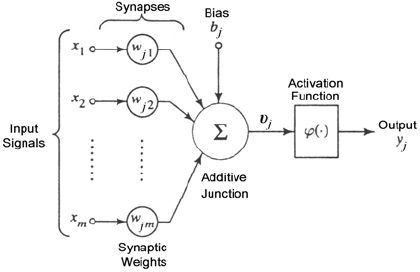
\includegraphics[width=0.55 \textwidth]{c.png}
    	\caption{Artificial Neuron Models and it's parts}
    	\label{fig:mesh3}
    	Adapted from hykin 
	\end{figure}   
	
 figure \ref{fig:mesh3}   Shows the basic structure of a simple artificial neural network. Here, $x_1,x_2,... x_n$ Represents the inputs to the neural network. $w_{j_1}, w_{j_2}, w_{j_3},..., w_{j_m}$ are the respective weights of neurons weights.It also includes an externally applied bias, denoted by $b_j$.The bias $b_j$ has the effect of increasing or lowering the net input of the activation function, depending on whether it is positive or negative, respectively. 
 \newpage
 In mathematical term. 
 
 \begin{equation}
 u_j=\sum_{i=1}^{m} w{j_i}*x_i= 1
 \end{equation}
 
 And
 
 \begin{equation}
    y_j= \varphi(v_j+b_j)
 \end{equation}
 where
 \begin{equation}
    v_j=u_j+b_j
    \label{mesh:eq3}
 \end{equation}
 
 $\varphi$ is the activation function; and $y_j$ is the output signal of the neuron. The use of bias $b_j$ has the effect of applying an affine transformation to the output $u_j$ of the linear combiner in the model as shown in equation \ref{mesh:eq3}
 
 The activation function, denoted by $\varphi(v)$, defines the output of a neuron in terms of
the induced local field $v$. In what follows, we identify two basic types of activation functions: 
\vspace{2mm}
1. \textbf{Threshold Function}: For this type of activation function, described in Figure 4, we have 
	
\[
   \varphi(x)= 
\begin{cases}
    1 ,& \text{if\hspace{2mm} } v \geq 1 \\
       0,              & \text{if\hspace{2mm} }  \ v < 1
\end{cases}
\]
In engineering, this form of a threshold function is commonly referred to as a Heaviside
function.

In neural computation, such a neuron is referred to as the McCulloch–Pitts model, in
recognition of the pioneering work done by McCulloch and Pitts (1943). In this model,
the output of a neuron takes on the value of 1 if the induced local field of that neuron
is nonnegative, and 0 otherwise.This statement describes the all-or-none property of the
McCulloch–Pitts model
 \begin{figure}[h]
    	\centering
    	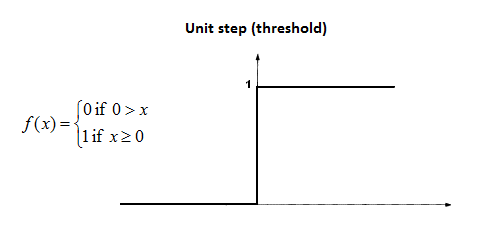
\includegraphics[width=0.35 \textwidth]{d.png}
       	\label{fig:mesh4}
	\caption{Unit step (Threshold function)}
	\end{figure} 
    \subsection{Neural network architectures}
    	\subsubsection{Feed forward neural network}
        The feedforward neural network was the first and arguably most simple type of artificial neural network devised. In this network the information moves in only one direction—forward: From the input nodes data goes through the hidden nodes  (if  any)  and  to  the  output  nodes.  There  are  no  cycles  or  loops  in  the  network.  Feedforward  networks  can  be constructed  from  different  types  of  units,  e.g.  binary McCulloch
-
Pitts  neurons
,  the  simplest  example  being  the 
perceptron. Continuous  neurons,  frequently  with  sigmoidal activation, are  used  in  the  context  of 
back  propagation
of error.
        \subsubsection{Recurrent neural networks}

        Contrary  to feedforward  networks, recurrent  neural  networks(RNNs)  are  models  with  bidirectional  data  flow. While  a  feedforward  network  propagates  data  linearly  from  input  to  output,  RNNs  also  propagate  data  from  later processing stages to earlier stages. RNNs can be used as general sequence processors.
    \subsection{Machine learning processes}
    3 main types of learning processes are 
    
       \qquad \textbf{1.} Supervised learning
       
       \qquad \textbf{2.} Unsupervised learning
       
       \qquad\textbf{3.} Reinforced learning
       
       
        \subsubsection{Supervised learning}
        Supervised learning uses a set of example pairs $(x,y)$ , $x \in X , y \in Y$ and the aim is to find a function $f : X \rightarrow Y $ in the allowed class of functions that matches the examples. In other words, we wish to infer the mapping implied by the data; the cost function is related to the mismatch between our mapping and the data and it implicitly contains prior knowledge about the problem domain.

A commonly used cost is the mean-squared error, which tries to minimize the average squared error between the network's output, $f ( x )$  and the target value $y$ over all the example pairs. Minimizing this cost using gradient descent for the class of neural networks called multilayer perceptrons (MLP), produces the backpropagation algorithm for training neural networks.

Tasks that fall within the paradigm of supervised learning are pattern recognition (also known as classification) and regression (also known as function approximation). The supervised learning paradigm is also applicable to sequential data (e.g., for hand writing, speech and gesture recognition). This can be thought of as learning with a "teacher", in the form of a function that provides continuous feedback on the quality of solutions obtained thus far.
        \subsubsection{Unsupervised learning}
        In unsupervised learning, some data $x$ is given and the cost function to be minimized, that can be any function of the data $x$ and the network's output, $f$
        
The cost function is dependent on the task (the model domain) and any a priori assumptions (the implicit properties of the model, its parameters and the observed variables).

As a trivial example, consider the model $f ( x ) = a$  $f(x)=a$ where $a$ is a constant and the cost $C=E[(x-f(x))^2]$. Minimizing this cost produces a value of $\alpha$ that is equal to the mean of the data. The cost function can be much more complicated. Its form depends on the application: for example, in compression it could be related to the mutual information between $x$  and $f ( x )$ , whereas in statistical modeling, it could be related to the posterior probability of the model given the data (note that in both of those examples those quantities would be maximized rather than minimized).

Tasks that fall within the paradigm of unsupervised learning are in general estimation problems; the applications include clustering, the estimation of statistical distributions, compression and filtering.
        \subsubsection{Reinforced Learning}
        In reinforcement learning, data $t$ are usually not given, but generated by an agent's interactions with the environment. At each point in time $t$, the agent performs an action $y_t$ and the environment generates an observation $x_t$ and an instantaneous cost $c_t$, according to some (usually unknown) dynamics. The aim is to discover a policy for selecting actions that minimizes some measure of a long-term cost, e.g., the expected cumulative cost. The environment's dynamics and the long-term cost for each policy are usually unknown, but can be estimated.
        
        ANNs are frequently used in reinforcement learning as part of the overall algorithm. Dynamic programming was coupled with ANNs (giving neurodynamic programming) by Bertsekas and Tsitsiklis and applied to multi-dimensional nonlinear problems such as those involved in vehicle routing, natural resources management or medicine because of the ability of ANNs to mitigate losses of accuracy even when reducing the discretization grid density for numerically approximating the solution of the original control problems.
\section{\fontsize{14}{14}\selectfont Convolutional Neural Network}
\begin{figure}[h]
    	\centering
    	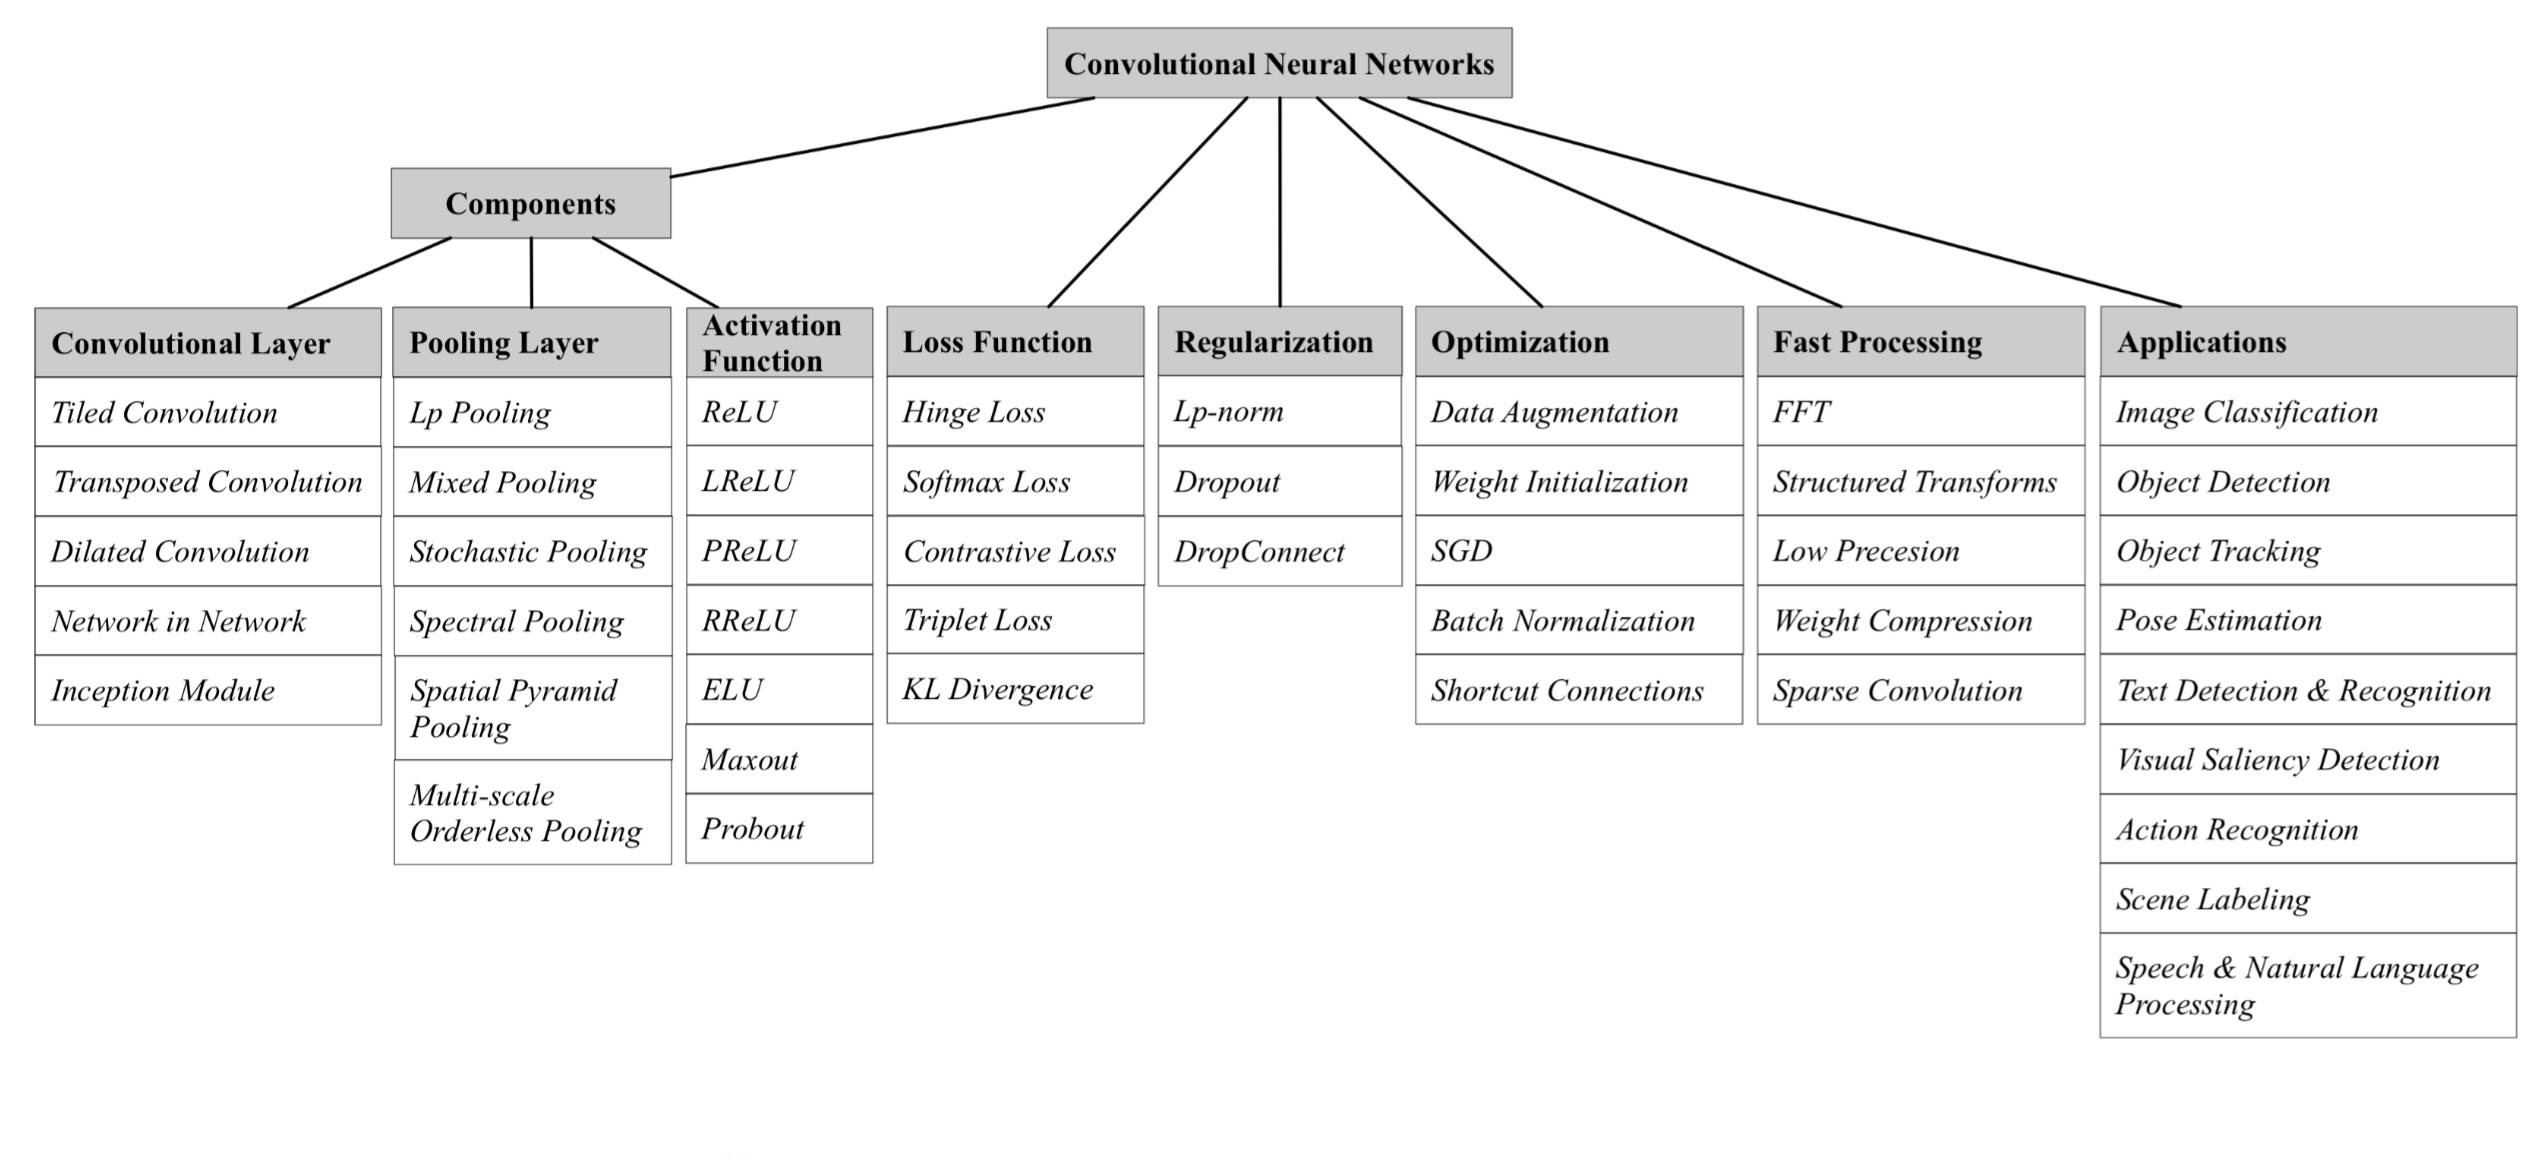
\includegraphics[width=1\textwidth]{cnn1.jpg}
       	\label{fig:mesh5}
	\caption{Convolutional neural network overview}
	\end{figure} 

    Some of the computer vision problems are yet to be solved and convolutional neural network has been the main point of interest in this field for the last 4-5 years. Last month ( October 2017), Geoffray Hinton who is famous for his works in deep learning at google, Introduced a new concept called Capsule Neural network. The only competition to ConvNet is still too young and under development. This report is to give the readers a good introduction to ConvNet and guide them through each steps to implement CNN. When we look into the hystory of CNN, It started back in the early 1998. But the lack of computational power restricted the researchers in doing more in the field of computer vision. Also the introduction of Deep learning concepts and availability of powerful CPUs and GPUs made people use ConvNets more in the field of computer vision. 

\begin{figure}[h]
    	\centering
    	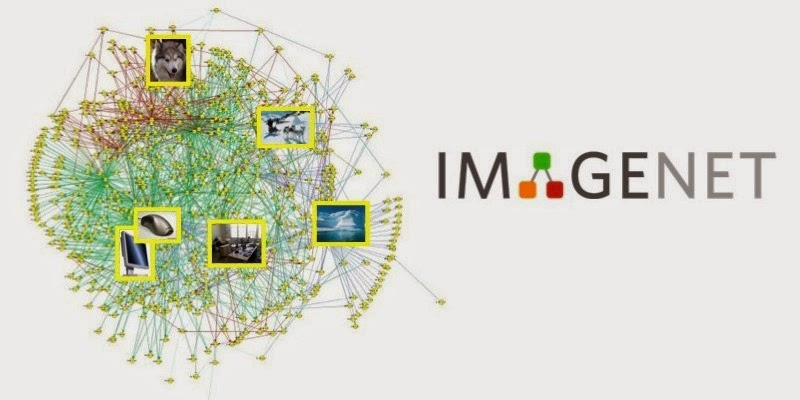
\includegraphics[width=0.75\textwidth]{e.jpg}
       	\label{fig:mesh6}
	\caption{ImageNet}
	\end{figure} 
    
ImageNet is a data set comprising of some 14 million images under 22,000 categories of objects. This was one of the biggest datasets made available during early 2010s and ImageNet Challenge was introduced just after the development of that dataset and from there on, it was used to identify the best image recognition/Object detection model in the world. Since 2012(SuperVision now AlexNet), all the models that won the ImageNet challenge were all convolutional neural network based models. Now the error rate has decreased so much that these models shows a better accuracy than human beings (Figure 6 - ResNet in 2015). 
\begin{figure}[h]
    	\centering
    	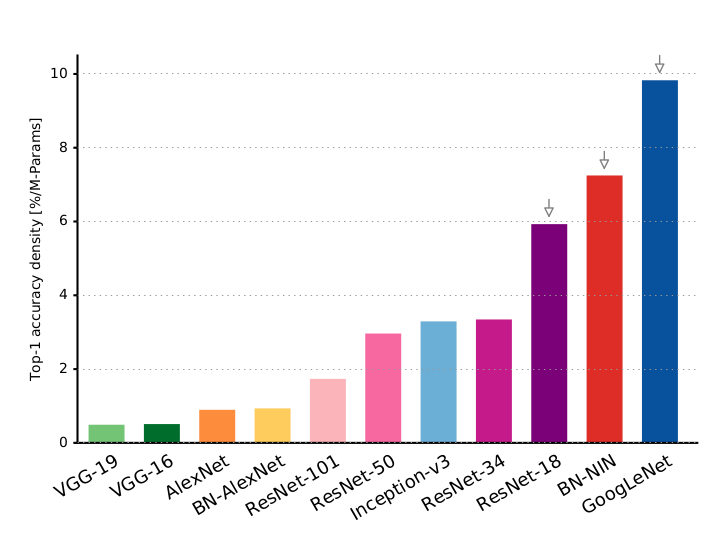
\includegraphics[width=0.75 \textwidth]{f.png}
       	\label{fig:mesh7}
	\caption{Winners of ImageNet challenge}
	\end{figure} 
    
    Alex krizhevsky is the one who used CNN in 2012 to win the ImageNet challenge. AlexNet showed an accuracy of 12\% which was a big change from 25.6\% in 2011. This was the point where the CNN buzz started and now in 2017, CNN is the most recognized computer vision model. 
    
    \subsection{The architecture}
    
    A convolutional network is a multilayer perceptron designed specifically to recognize two-dimensional shapes with a high degree of invariance to translation, scaling, skewing, and other forms of distortion.This difficult task is learned in a supervised manner by means of a network.
    
    A CNN usually takes an order 3 tensor as its input, e.g., an image with $H$ rows, $W$ columns, and 3 channels (R, G, B color channels). Higher order tensor inputs, however, can be handled by CNN in a similar fashion. The input then sequentially goes through a series of processing. One processing step is usually called a layer, which could be a convolution layer, a pooling layer, a normalization layer, a fully connected layer, a loss layer, etc.
    
    A convolutional network is a multilayer perceptron designed specifically to recognize
two-dimensional shapes with a high degree of invariance to translation, scaling, skewing, and other forms of distortion.This difficult task is learned in a supervised manner by means of a network whose structure includes the following forms of constraints
  
\quad 1. \textit{Feature extraction}. Each neuron takes its synaptic inputs from a local receptive
field in the previous layer, thereby forcing it to extract local features. Once a feature
has been extracted, its exact location becomes less important, so long as its position relative
to other features is approximately preserved.

    \quad 2. \textit{Feature mapping.}: Each computational layer of the network is composed of multiple feature maps, with each feature map being in the form of a plane within which the individual neurons are constrained to share the same set of synaptic weights. This second form of structural constraint has the following beneficial effects:
    \begin{itemize}
  \item \textit{shift invariance}, forced into the operation of a feature map through the use of \textit{convolution} with a kernel of small size, followed by a sigmoid function;
  \item reduction in the number of free parameters, accomplished through the use of weight sharing.
\end{itemize}
    
    \quad 3. \textit{Subsampling}. Each convolutional layer is followed by a computational layer that performs local averaging and subsampling, whereby the resolution of the feature map is reduced. This operation has the effect of reducing the sensitivity of the feature map’s output to shifts and other forms of distortion.
    
    We emphasize that all weights in all layers of a convolutional network are learned through training. Moreover, the network learns to extract its own features automatically.
    
    \begin{figure}[h]
    	\centering
    	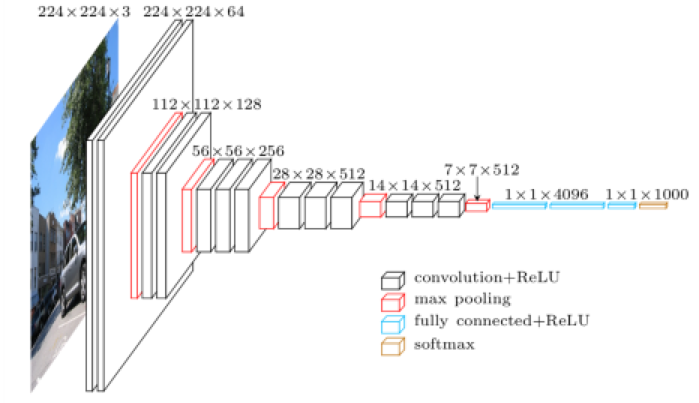
\includegraphics[width=0.75 \textwidth]{cnn.png}
       	\label{fig:mesh8}
	\caption{Architecture of Convolutional neural network }
	\end{figure} 
    
    Figure 8. Shows the basic structure of a convolutional neural network with 10 layers. Here the first one is the input layer which is the input 2D image with color as the 3rd parameter. the image is $224\times224\times3$. Here 3 represents the 3 channels. The images are in color, so they have three channels: red, green and blue. This image has a total $of 224\times224\times3 = 150,528$ features. the second layer is the convolution layer, in which the number of pixels remains the same but the number of features output is $224\times224\times64$. To reduce the amount of features, max pooling layer is applied and the output is $112\times112\times128$ and this continues several times depending on the design of the network. Fully connected layers stretch the data out to a one dimensional data. With the successive computational layers alternating between convolution and subsampling, we get a “bipyramidal” effect. That is, at each convolutional or subsampling layer, the number of feature maps is increased while the spatial resolution is reduced, compared with the corresponding previous layer.The idea of convolution followed by subsampling is inspired by the notion of “simple” cells followed by “complex” cells14, which is the parameter that plays a vital role in the detection of object. Here, 
    \begin{small}
    
\vspace{2mm}INPUT: [224x224x3]        memory:  224*224*3=150K   weights: 0

CONV3-64: [224x224x64]  memory:  224*224*64=3.2M   weights: (3*3*3)*64 = 1,728

CONV3-64: [224x224x64]  memory:  224*224*64=3.2M   weights: (3*3*64)*64 = 36,864

POOL2: [112x112x64]  memory:  112*112*64=800K   weights: 0

CONV3-128: [112x112x128]  memory:  112*112*128=1.6M   weights: (3*3*64)*128 = 73,728

CONV3-128: [112x112x128]  memory:  112*112*128=1.6M   weights: (3*3*128)*128 = 147,456

POOL2: [56x56x128]  memory:  56*56*128=400K   weights: 0

CONV3-256: [56x56x256]  memory:  56*56*256=800K   weights: (3*3*128)*256 = 294,912

CONV3-256: [56x56x256]  memory:  56*56*256=800K   weights: (3*3*256)*256 = 589,824

CONV3-256: [56x56x256]  memory:  56*56*256=800K   weights: (3*3*256)*256 = 589,824

POOL2: [28x28x256]  memory:  28*28*256=200K   weights: 0

CONV3-512: [28x28x512]  memory:  28*28*512=400K   weights: (3*3*256)*512 = 1,179,648

CONV3-512: [28x28x512]  memory:  28*28*512=400K   weights: (3*3*512)*512 = 2,359,296

CONV3-512: [28x28x512]  memory:  28*28*512=400K   weights: (3*3*512)*512 = 2,359,296

POOL2: [14x14x512]  memory:  14*14*512=100K   weights: 0

CONV3-512: [14x14x512]  memory:  14*14*512=100K   weights: (3*3*512)*512 = 2,359,296

CONV3-512: [14x14x512]  memory:  14*14*512=100K   weights: (3*3*512)*512 = 2,359,296

CONV3-512: [14x14x512]  memory:  14*14*512=100K   weights: (3*3*512)*512 = 2,359,296

POOL2: [7x7x512]  memory:  7*7*512=25K  weights: 0

FC: [1x1x4096]  memory:  4096  weights: 7*7*512*4096 = 102,760,448

FC: [1x1x4096]  memory:  4096  weights: 4096*4096 = 16,777,216

FC: [1x1x1000]  memory:  1000 weights: 4096*1000 = 4,096,000 
    
    \end{small}
    
     This is the specifications of this convolutional neural network shown in the image
     \subsection{Multi layer perceptron}
     \begin{figure}[h]
    	\centering
    	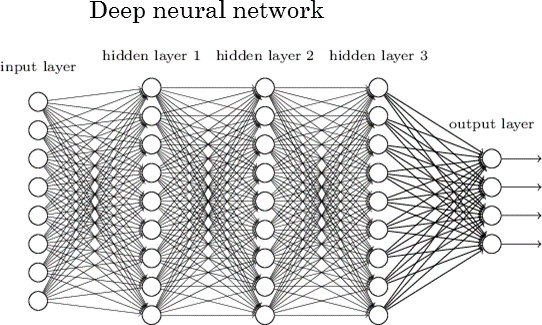
\includegraphics[width=0.55 \textwidth]{h.png}
    	\caption{Multi layer perceptron}
    	\label{fig:mesh9}
    	
	\end{figure}   
     
     
     Figure 9 shows the architectural graph of a multiplayer perceptron with three hidden
layers and an output layer. To set the stage for a description of the multilayer perceptron
in its general form, the network shown here is fully connected.This means that a neuron
in any layer of the network is connected to all the neurons (nodes) in the previous
layer. Signal flow through the network progresses in a forward direction, from left to right
and on a layer-by-layer basis. In the case of Convolutional neural networks, the connections are based on the number of features and strands. 

To overcome
the practical limitations of the perceptron and the LMS algorithm, we look to a neural
network structure known as the multilayer perceptron. An MLP have two terms that associates with it that makes them perform well. The main one is the concept of back propagation.
    \subsubsection{The forward run}
    In the forward phase, the synaptic weights of the network are fixed and the input signal is propagated through the network, layer by layer, until it reaches the output.
Thus, in this phase, changes are confined to the activation potentials and outputs of the neurons in the network

A function signal is an input signal (stimulus) that comes in at the input end of the network, propagates forward (neuron by neuron) through the network, and emerges at the output end of the network as an output signal.We refer to such a signal as a “function signal” for two reasons. First, it is presumed to
perform a useful function at the output of the network. Second, at each neuron of the network through which a function signal passes, the signal is calculated as a function of the inputs and associated weights applied to that neuron.The function signal is also referred to as the input signal.
    \subsubsection{Back propagation}
    
    In the backward phase, an error signal is produced by comparing the output of the network with a desired response.The resulting error signal is propagated through
the network, again layer by layer, but this time the propagation is performed in the backward direction. In this second phase, successive adjustments are made to the
synaptic weights of the network. Calculation of the adjustments for the output layer is straightforward, but it is much more challenging for the hidden layers.

An error signal originates at an output neuron of the network and propagates backward (layer by layer) through the network.We refer to it as an “error signal” because its computation by every neuron of the network involves an
error-dependent function in one form or another. Stochastic gradient descent (SGD) is used in convolutional neural networks since the parameters of a CNN model are optimized to minimize the loss $z$, i.e., we want the prediction of a CNN model to match the ground truth labels.
    \subsection{Layer, input, output and notation}
		    
    Now that the CNN architecture is clear, we will discuss in detail the different types of layers, starting from the Convolution layer, which is the simplest layer among
those we discuss in this report.
\begin{figure}[h]
    	\centering
    	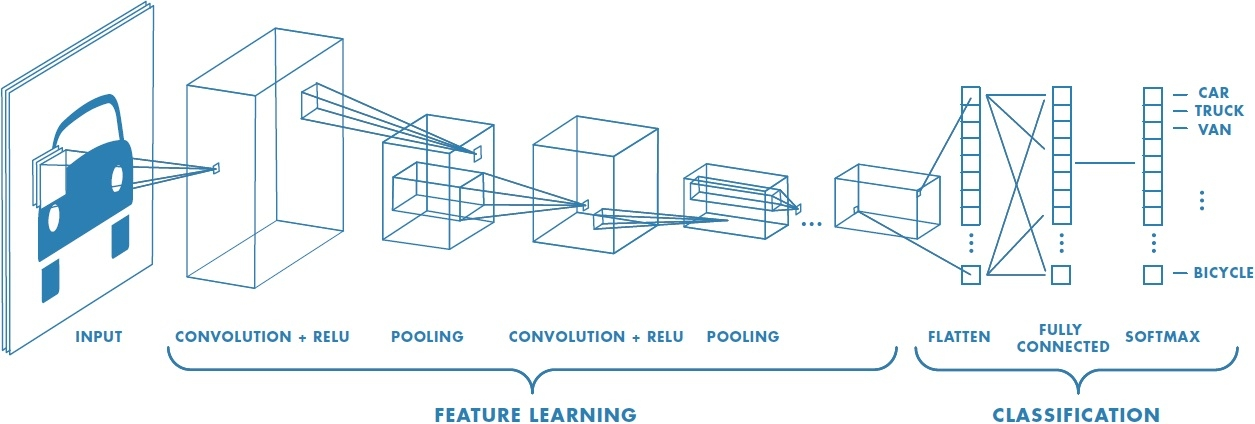
\includegraphics[width=0.75\textwidth]{cnn2.jpg}
       	\label{fig:mesh10}
	\caption{ConvNet}
	\end{figure} 

        \subsubsection{Convolution layer}
		
		 Lets first discuss what the CONV layer computes without brain/neuron analogies. The CONV layer’s parameters consist of a set of learnable filters. Every filter is small spatially (along width and height), but extends through the full depth of the input volume. For example, a typical filter on a first layer of a ConvNet might have size 5x5x3 (i.e. 5 pixels width and height, and 3 because images have depth 3, the color channels).
\begin{figure}[h]
    	\centering
    	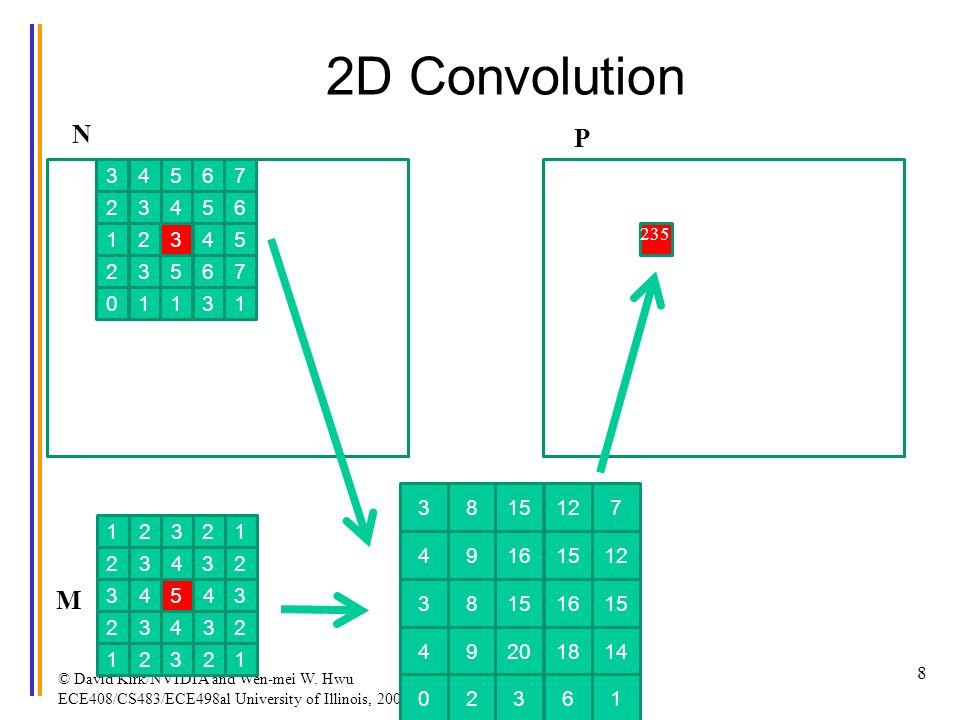
\includegraphics[width=0.75\textwidth]{2d.jpg}
       	\label{fig:mesh11}
	\caption{Convolution}
	\end{figure}

		 
		  During the forward pass, we slide (more precisely, convolve) each filter across the width and height of the input volume and compute dot products between the entries of the filter and the input at any position. As we slide the filter over the width and height of the input volume we will produce a 2-dimensional activation map that gives the responses of that filter at every spatial position. Intuitively, the network will learn filters that activate when they see some type of visual feature such as an edge of some orientation or a block of some color on the first layer, or eventually entire honeycomb or wheel-like patterns on higher layers of the network. Now, we will have an entire set of filters in each CONV layer (e.g. 12 filters), and each of them will produce a separate 2-dimensional activation map. We will stack these activation maps along the depth dimension and produce the output volume.
		         
        
        \begin{figure}[h]
    	\centering
    	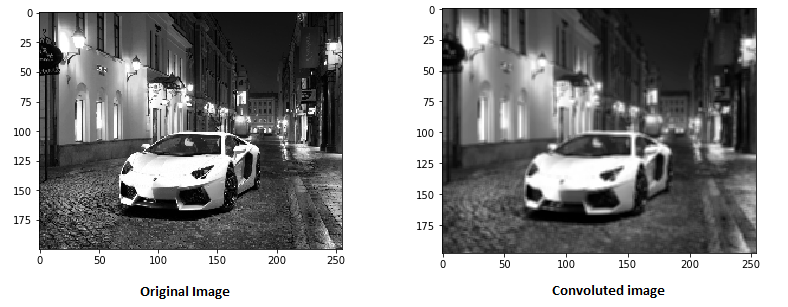
\includegraphics[width=0.75\textwidth]{convimages.png}
       	\label{fig:mesh12}
	\caption{Convolution}
	\end{figure} 
	
	\subsubsection{ReLu layer}
 \begin{figure}[h]
    	\centering
    	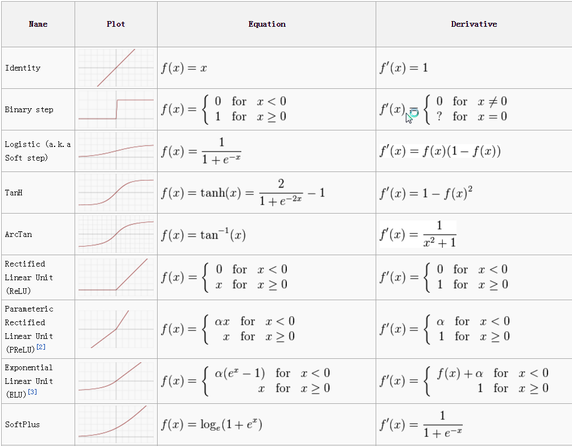
\includegraphics[width=1\textwidth]{act.png}
       	\label{fig:mesh13}
	\caption{ReLu}
	\end{figure} 

After each conv layer, it is convention to apply a non-linear layer (or activation layer) immediately afterwards.The purpose of this layer is to introduce non-linearity to a system that basically has just been computing linear operations during the conv layers (just element wise multiplications and summations).In the past, non-linear functions like tanh and sigmoid were used, but researchers found out that ReLU layers work far better because the network is able to train a lot faster (because of the computational efficiency) without making a significant difference to the accuracy.

 It also helps to alleviate the vanishing gradient problem, which is the issue where the lower layers of the network train very slowly because the gradient decreases exponentially through the layers (Explaining this might be out of the scope of this post, but see here and here for good descriptions). The ReLU layer applies the function $f(x) = max(0, x)$ to all of the values in the input volume. In basic terms, this layer just changes all the negative activations to 0.This layer increases the nonlinear properties of the model and the overall network without affecting the receptive fields of the conv layer.
        
        \subsubsection{Pooling layer}
         After some ReLU layers, programmers may choose to apply a pooling layer. It is also referred to as a downsampling layer. In this category, there are also several layer options, with maxpooling being the most popular. This basically takes a filter (normally of size 2x2) and a stride of the same length. It then applies it to the input volume and outputs the maximum number in every subregion that the filter convolves around.
         
          Other options for pooling layers are average pooling and L2-norm pooling. The intuitive reasoning behind this layer is that once we know that a specific feature is in the original input volume (there will be a high activation value), its exact location is not as important as its relative location to the other features. As you can imagine, this layer drastically reduces the spatial dimension (the length and the width change but not the depth) of the input volume. This serves two main purposes. The first is that the amount of parameters or weights is reduced by 75\%, thus lessening the computation cost. The second is that it will control overfitting. This term refers to when a model is so tuned to the training examples that it is not able to generalize well for the validation and test sets. A symptom of overfitting is having a model that gets 100\% or 99\% on the training set, but only 50\% on the test data.
         
          \begin{figure}[h]
    	\centering
    	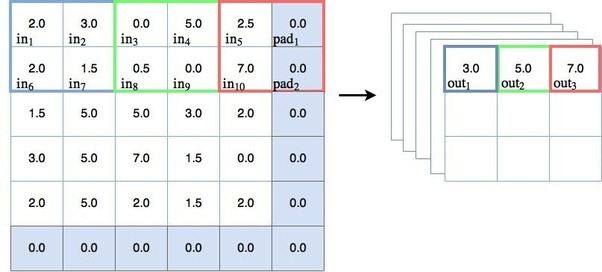
\includegraphics[width=0.75\textwidth]{popo.jpg}
       	\label{fig:mesh14}
	\caption{Pooling}
	\end{figure} 
         
               
        \begin{figure}[h]
    	\centering
    	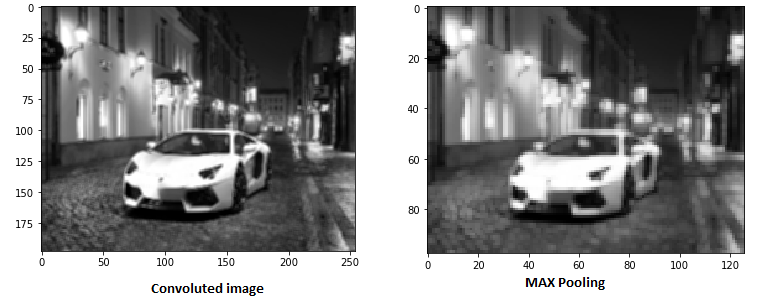
\includegraphics[width=0.75\textwidth]{pooling.png}
       	\label{fig:mesh15}
	\caption{Pooling results}
	\end{figure} 
	
		
	
        \subsubsection{Fully connected layer }
        Dense (fully connected) layers, which perform classification on the features extracted by the convolutional layers and downsampled by the pooling layers. In a dense layer, every node in the layer is connected to every node in the preceding layer

 FC and CONV layers is that the neurons in the CONV layer are connected only to a local region in the input, and that many of the neurons in a CONV volume share parameters. However, the neurons in both layers still compute dot products, so their functional form is identical. Therefore, it turns out that it’s possible to convert between FC and CONV layers.
\section{\fontsize{14}{14}\selectfont Tools for object detection using CNN and basic implementation}
Requirements:


1. Basic knowledge in Python

2. Basic knowledge in Tensorflow

3. Images to be trained (Here we will be using MNIST DATASET)

Components in the following code

\begin{itemize}

   \item Convolutional Layer \#1: Applies 32 5x5 filters (extracting 5x5-pixel subregions), with ReLU activation function
   \item Pooling Layer \#1: Performs max pooling with a 2x2 filter and stride of 2 (which specifies that pooled regions do not overlap)
   \item Convolutional Layer \#2: Applies 64 5x5 filters, with ReLU activation function
   \item Pooling Layer \#2: Again, performs max pooling with a 2x2 filter and stride of 2
   \item Dense Layer(Fully connected) \#1: 1,024 neurons, with dropout regularization rate of 0.4 (probability of 0.4 that any given element will be dropped during training)
    \item Dense Layer \#2 (Logits Layer): 10 neurons, one for each digit target class (0–9).
    
\end{itemize}


Code\footnote{The code is self explanatory. For further information, visit Tensorflow website}:
\begin{lstlisting}[language=python]
def cnn_model_fn(features, labels, mode):
  """Model function for CNN."""
  # Input Layer
  input_layer = tf.reshape(features["x"], [-1, 28, 28, 1])

  # Convolutional Layer #1
  conv1 = tf.layers.conv2d(
      inputs=input_layer,
      filters=32,
      kernel_size=[5, 5],
      padding="same",
      activation=tf.nn.relu)

  \# Pooling Layer #1
  pool1 = tf.layers.max_pooling2d(inputs=conv1, pool_size=[2, 2], strides=2)

  # Convolutional Layer #2 and Pooling Layer #2
  conv2 = tf.layers.conv2d(
      inputs=pool1,
      filters=64,
      kernel_size=[5, 5],
      padding="same",
      activation=tf.nn.relu)
  pool2 = tf.layers.max_pooling2d(inputs=conv2, pool_size=[2, 2], strides=2)

  # Dense Layer
  pool2_flat = tf.reshape(pool2, [-1, 7 * 7 * 64])
  dense = tf.layers.dense(inputs=pool2_flat, units=1024, activation=tf.nn.relu)
  dropout = tf.layers.dropout(
      inputs=dense, rate=0.4, training=mode == tf.estimator.ModeKeys.TRAIN)

  # Logits Layer
  logits = tf.layers.dense(inputs=dropout, units=10)

  predictions = {
      # Generate predictions (for PREDICT and EVAL mode)
      "classes": tf.argmax(input=logits, axis=1),
      # Add `softmax_tensor` to the graph. It is used for PREDICT and by the
      # `logging_hook`.
      "probabilities": tf.nn.softmax(logits, name="softmax_tensor")
  }

  if mode == tf.estimator.ModeKeys.PREDICT:
    return tf.estimator.EstimatorSpec(mode=mode, predictions=predictions)

  # Calculate Loss (for both TRAIN and EVAL modes)
  onehot_labels = tf.one_hot(indices=tf.cast(labels, tf.int32), depth=10)
  loss = tf.losses.softmax_cross_entropy(
      onehot_labels=onehot_labels, logits=logits)

  # Configure the Training Op (for TRAIN mode)
  if mode == tf.estimator.ModeKeys.TRAIN:
    optimizer = tf.train.GradientDescentOptimizer(learning_rate=0.001)
    train_op = optimizer.minimize(
        loss=loss,
        global_step=tf.train.get_global_step())
    return tf.estimator.EstimatorSpec(mode=mode, loss=loss, train_op=train_op)

  # Add evaluation metrics (for EVAL mode)
  eval_metric_ops = {
      "accuracy": tf.metrics.accuracy(
          labels=labels, predictions=predictions["classes"])}
  return tf.estimator.EstimatorSpec(
      mode=mode, loss=loss, eval_metric_ops=eval_metric_ops)
\end{lstlisting}



    \subsection{Meta architectures}
        \subsubsection{SSD}
        \begin{figure}[h]
    	\centering
    	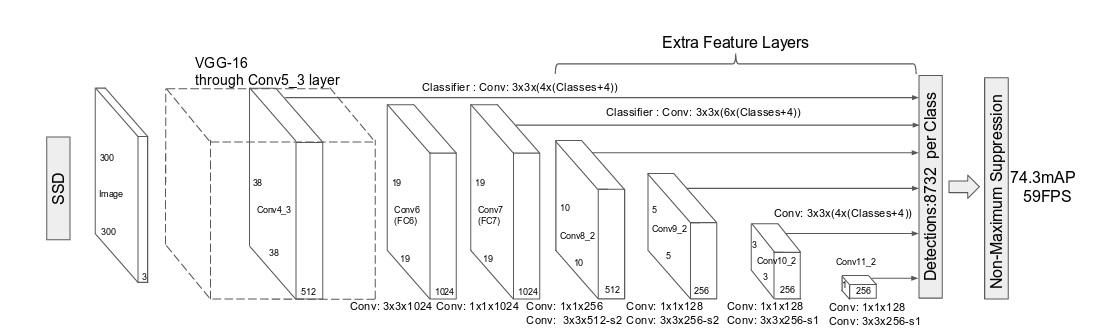
\includegraphics[width=1\textwidth]{ssd.png}
       	\label{fig:mesh16}
	\caption{ssd}
	\end{figure} 
        Single shot Multi box detector is a method for detecting objects in images using a single deep neural network. Our approach, named SSD, discretizes the output space of bounding boxes into a set of default boxes over different aspect ratios and scales per feature map location. At prediction time, the network generates scores for the
presence of each object category in each default box and produces adjustments to
the box to better match the object shape. Additionally, the network combines predictions from multiple feature maps with different resolutions to naturally handle objects of various sizes. SSD is simple relative to methods that require object proposals because it completely eliminates proposal generation and subsequent pixel or feature resampling stages and encapsulates all computation in a single network. This makes SSD easy to train and straightforward to integrate into systems that require a detection component. Experimental results on the PASCAL VOC, COCO, and ILSVRC datasets confirm that SSD has competitive accuracy to methods that utilize an additional object proposal step and is much faster, while
providing a unified framework for both training and inference. For $300\times 300$ input, SSD achieves 74.3\% $mAP$
on VOC2007 test at 59 FPS on a Nvidia TitanX and for
$512\times 512$ input, SSD achieves 76.9\% $mAP$, outperforming a comparable state-of-the-art Faster R-CNN model. Compared to other single stage methods, SSD has much better accuracy even with a smaller input image size
        
        \subsubsection{Fast R-CNN}
        Recently, deep ConvNets have significantly improved image classification and object detection
accuracy.  Compared to image classification, object detection  is  a  more  challenging  task  that  requires  more  complex methods to solve.  Due to this complexity, current approaches, train models in multi-stage pipelines that are slow and inelegant. Complexity  arises  because  detection  requires  the  accurate  localization  of  objects,  creating  two  primary  challenges.   First,  numerous  candidate  object  locations  (often called “proposals”) must be processed.  Second, these candidates provide only rough localization that must be refined to achieve precise localization. Solutions to these problems often compromise speed, accuracy, or simplicity.
In this methode, they streamline the training process for state-of-the-art ConvNet-based object detectors in the paper[9].  Fat R-CNN propose a single-stage training algorithm that jointly learns to
classify object proposals and refine their spatial locations.
The  resulting  method  can  train  a  very  deep  detection
network (VGG16) 9 × faster than R-CNN and 3 × faster than SPPnet .  At runtime, the detection network
processes images in 0.3s (excluding object proposal time)
while achieving top accuracy on PASCAL VOC 2012 
with a $mAP$ of 66\% (vs. 62\% for R-CNN)
        
        \subsubsection{ R-FCN }
        
R-FCN \footnote{Code is made publicly available at: \url{ https://github.com/daijifeng001/r-fcn}.} present region-based, fully convolutional networks for accurate and efficient
object detection. In contrast to previous region-based detectors such as Fast/Faster R-CNN that apply a costly per-region subnetwork hundreds of times, our
region-based detector is fully convolutional with almost all computation shared on the entire image. To achieve this goal, we propose position-sensitive score maps to address a dilemma between translation-invariance in image classification and
translation-variance in object detection. Our method can thus naturally adopt fully convolutional image classifier backbones, such as the latest Residual Networks (ResNets) for object detection. We show competitive results on the PASCAL
VOC  datasets  (e.g.,  83.6\%  mAP  on  the  2007  set) with  the  101-layer  ResNet. Meanwhile, our result is achieved at a test-time speed of 170ms per image, 2.5-20× faster than the Faster R-CNN counterpart.         
        
    \subsection{Feature extractors}
    There are several architectures in the field of Convolutional Networks that have a name.
    \begin{figure}[h]
    	\centering
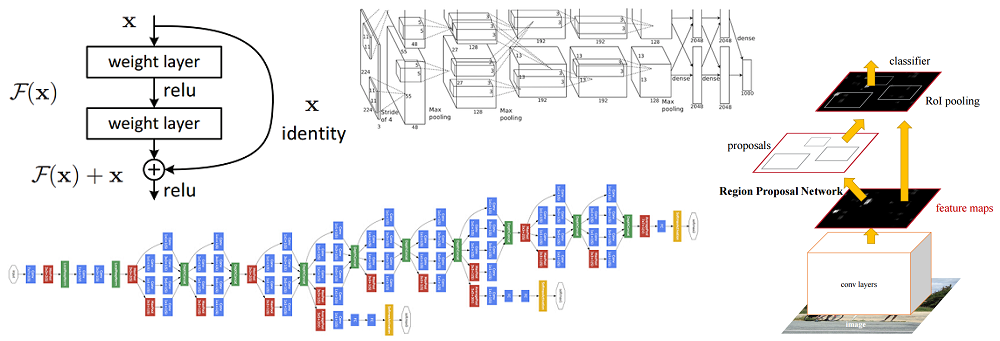
\includegraphics[width=1\textwidth]{ince.png}
       	\label{fig:mesh17}
	 	 \caption{Different extractors}
	\end{figure} 
	     The most common are:
    
        \subsubsection{GoogleNet}
        GoogLeNet. The ILSVRC 2014 winner was a Convolutional Network from Szegedy et al. from Google. Its main contribution was the development of an Inception Module that dramatically reduced the number of parameters in the network (4M, compared to AlexNet with 60M). Additionally, this paper uses Average Pooling instead of Fully Connected layers at the top of the ConvNet, eliminating a large amount of parameters that do not seem to matter much. There are also several followup versions to the GoogLeNet, most recently Inception-v4.
        \begin{figure}[h]
    	\centering
        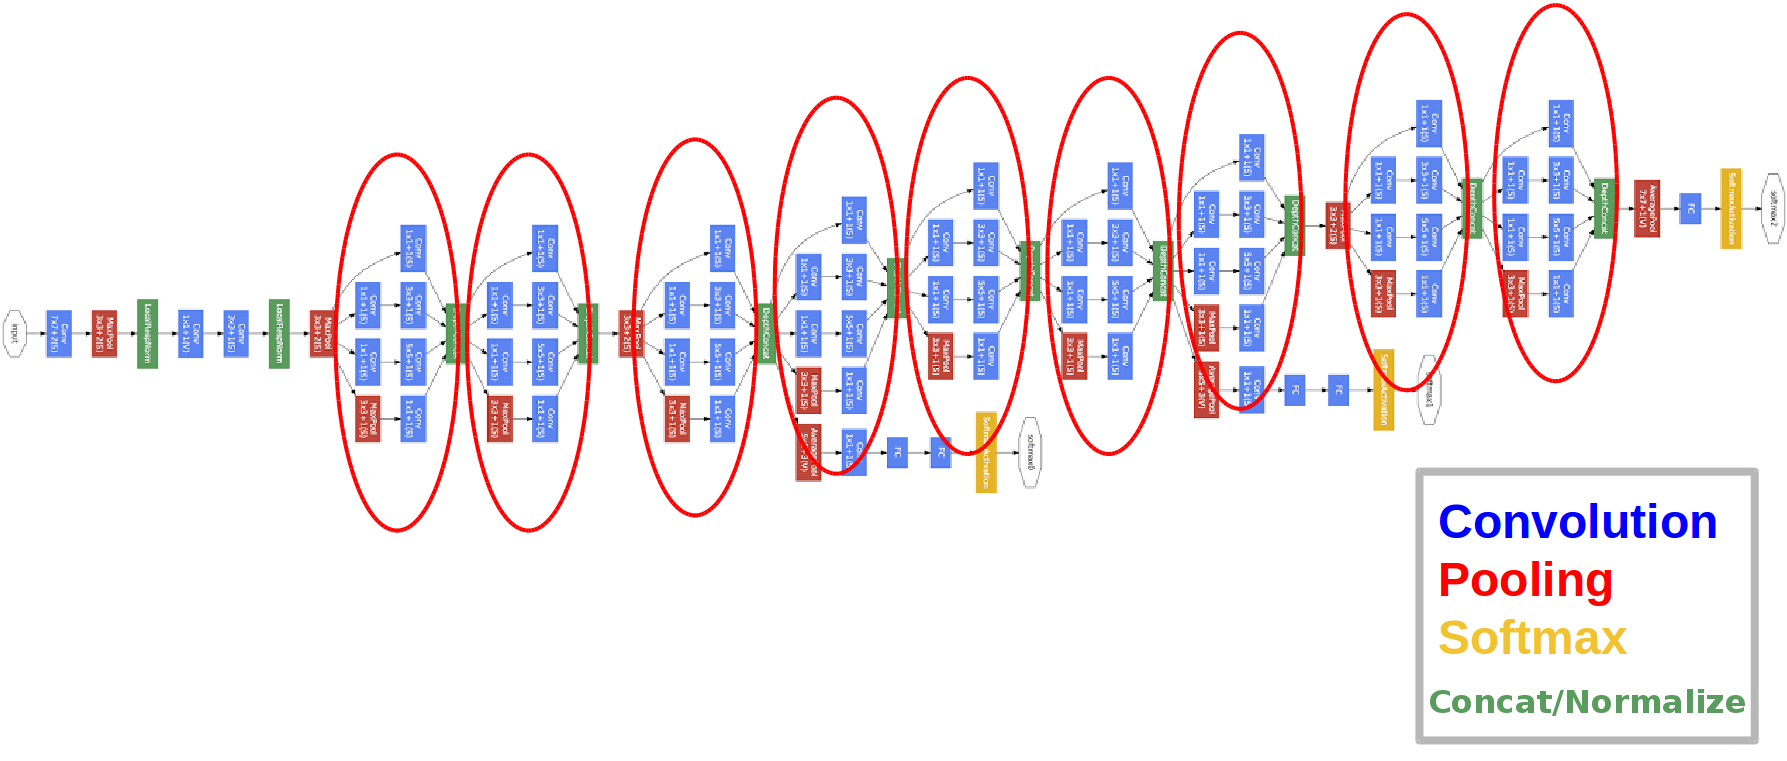
\includegraphics[width=1\textwidth]{gnet.png}
       	\label{fig:mesh18}
	\caption{GoogleNet(Inception 4)}
	\end{figure} 
        
       Very deep convolutional networks have been central to
the largest advances in image recognition performance in
recent years. One example is the Inception architecture that
has been shown to achieve very good performance at relatively low computational cost.  Recently, the introduction
of residual connections in conjunction with a more traditional architecture has yielded state-of-the-art performance
in the 2015 ILSVRC challenge; its performance was similar
to the latest generation Inception-v3 network.  This raises
the question of whether there are any benefit in combining
the Inception architecture with residual connections.  Here
we give clear empirical evidence that training with residual
connections accelerates the training of Inception networks
significantly. There is also some evidence of residual Inception networks outperforming similarly expensive Inception
networks without residual connections by a thin margin. It
also present several new streamlined architectures for both
residual and non-residual Inception networks. These variations improve the single-frame recognition performance on
the ILSVRC 2012 classification task significantly.  We further demonstrate how proper activation scaling stabilizes
the training of very wide residual Inception networks. With
an  ensemble  of  three  residual  and  one  Inception-v4,  It
achieved 3.08\% top-5 error on the test set of the ImageNet
classification (CLS) challenge. Human error is 5.7\%.
        \subsubsection{MobileNet}

        They present a class of efficient models called MobileNets for mobile and embedded vision applications.  MobileNets are  based  on  a  streamlined  architecture  that  uses  depth wise  separable  convolutions  to  build  light  weight  deep neural  networks.   They  introduced  two  simple  global  hyper parameters  that  efficiently  trade  off  between  latency  and accuracy. These hyper-parameters allow the model builder to choose the right sized model for their application based on  the  constraints  of  the  problem.   We  present  extensive experiments on resource and accuracy tradeoffs and show strong performance compared to other popular models on ImageNet classification.It's use  cases  including  object  detection,  finegrain  classification, face attributes and large scale geo-localization.
        
        \subsubsection{ResNet}

ResNet is a short name for Residual Network. As the name of the network indicates, the new terminology that this network introduces is residual learning.


Deep convolutional neural networks have led to a series of breakthroughs for image classification. Many other visual recognition tasks have also greatly benefited from very deep models. So, over the years there is a trend to go more deeper, to solve more complex tasks and to also increase /improve the classification/recognition accuracy. But, as we go deeper; the training of neural network becomes difficult and also the accuracy starts saturating and then degrades also. Residual Learning tries to solve both these problems.

\begin{figure}[h]
    	\centering
    	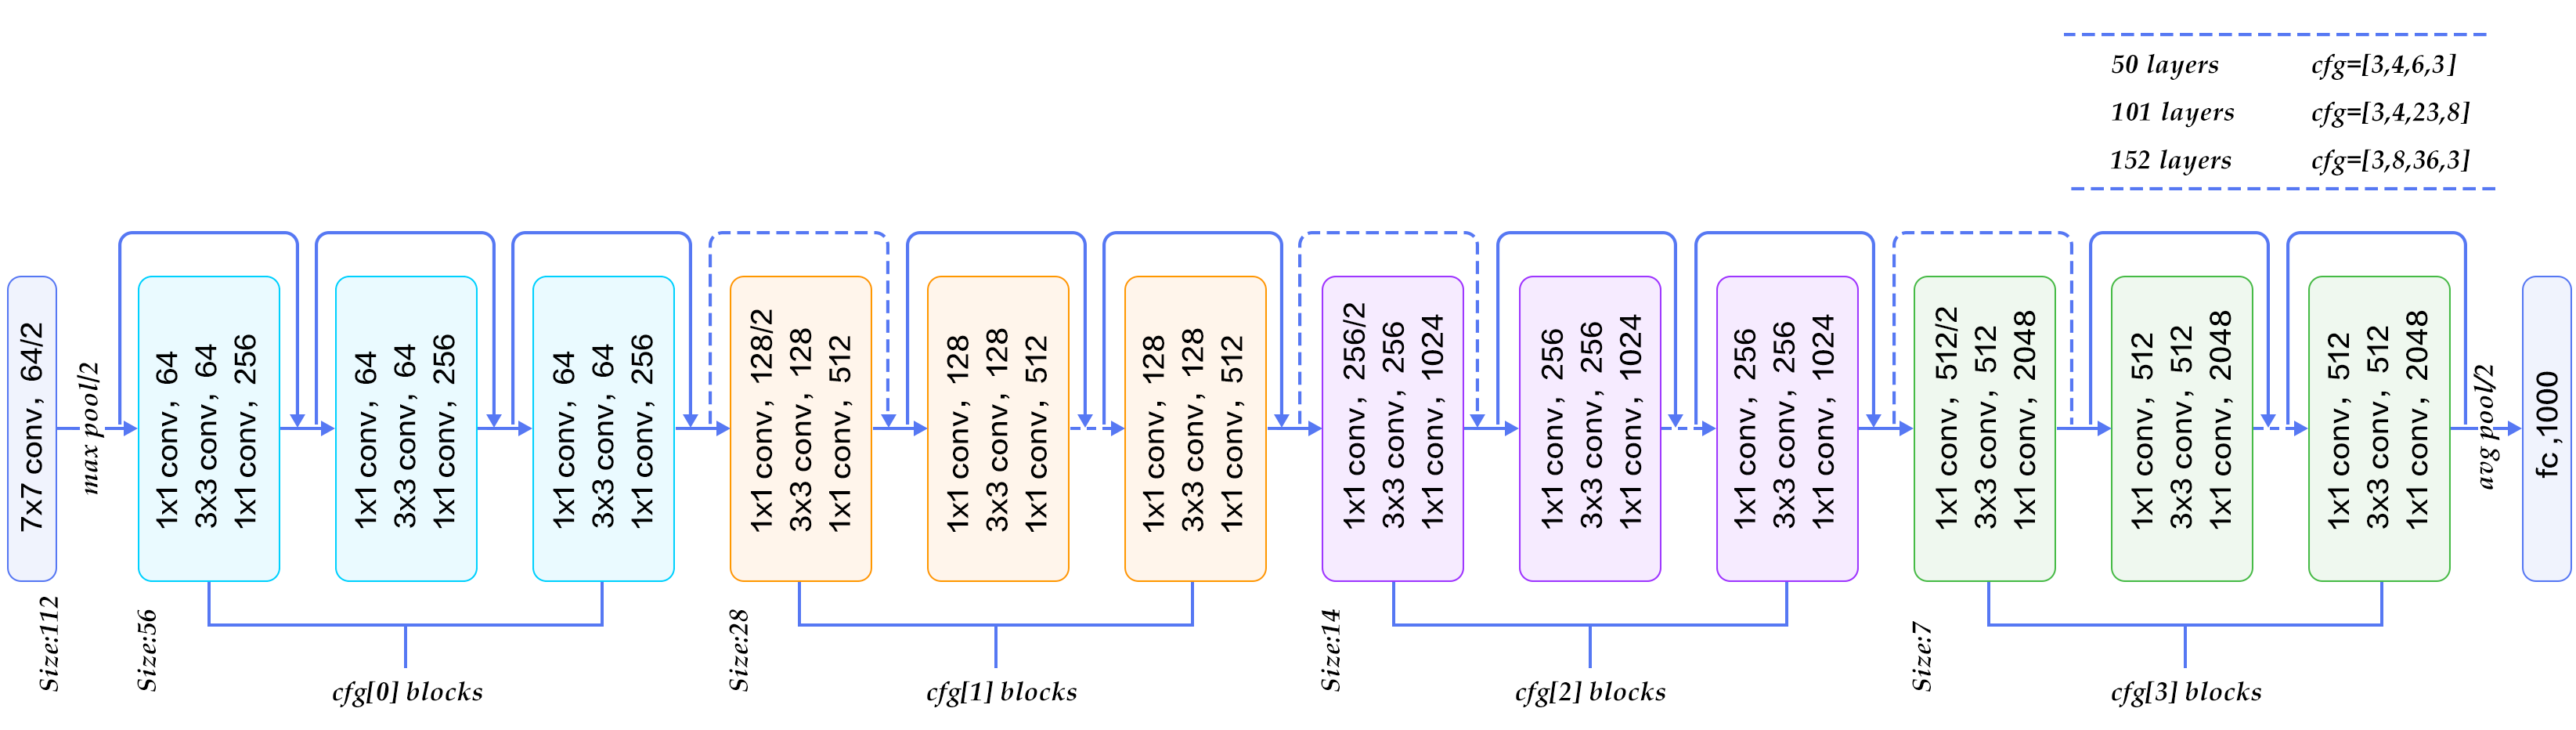
\includegraphics[width=1\textwidth]{resnet.png}
       	\label{fig:mesh19}
	 	 \caption{ResNet}
	\end{figure} 

In general, in a deep convolutional neural network, several layers are stacked and are trained to the task at hand. The network learns several low/mid/high level features at the end of its layers. In residual learning, instead of trying to learn some features, they try to learn some residual. Residual can be simply understood as subtraction of feature learned from input of that layer. ResNet does this using shortcut connections (directly connecting input of nth layer to some (n+x)th layer. It has proved that training this form of networks is easier than training simple deep convolutional neural networks and also the problem of degrading accuracy is resolved, This is the fundamental concept of ResNet.

ResNet50 is a 50 layer Residual Network. There are other variants like ResNet101 and ResNet152 also.        
        
\section{\fontsize{14}{14}\selectfont Applications of CNN}


A. Computer Vision

Convolutional neural networks are employed to identify
the hierarchy or conceptual structure of an image. Instead of
feeding each image into the neural network as one grid of
numbers, the image is broken down into overlapping image
tiles that are each fed into a small neural network.
Convolutional neural networks are trainable multi-stage
architectures,  with the inputs and outputs of each
stage consisting of sets of arrays called feature maps. If the
input is a colour image, each feature map is a 2D array
containing a colour channel of the input image, for a video
or a volumetric image it would be a 3D array. Each feature
extracted at all locations on the input is represented by a
feature map at the output. Each stage is composed of a filter
bank layer, a non-linearity layer and a feature pooling layer.
A typical CNN is composed of one, two or three such 3layer stages, followed by a classification module.

1) Face Recognition: Face recognition constitutes a
series of related problems
Identifying all the faces in the picture
Focussing on each face despite bad lighting or
different pose
Identifying unique features
Comparing identified features to existing database
and determining the person's name
Faces represent a complex, multi-dimensional, visual
stimulus which was earlier presented using a hybrid neural
network combining local image sampling, a self-organizing
map neural network and a convolutional neural network.
The results were presented using Karhunen-Loe`ve
transform in place of the self-organizing map which
performed almost as well (5.3\% error versus 3.8\%) and a
multi-layer perceptron which performed poorly (40\% error
versus 3.8\%). 

2) Scene Labelling: Each pixel is labelled with the
category of the object it belongs to in scene labelling.
Clement Farabet et al proposed a method using a multiscale
convolutional network that yielded record accuracies on the
Sift Flow Dataset (33 classes) and the Barcelona Dataset
(170 classes) and near-record accuracy on Stanford
Background Dataset (8 classes). Their method produced
320 X 240 image labelling in under a second including
feature extraction. 
Recurrent architecture  for convolutional neural
network suggests a sequential series of networks sharing the
same set of parameters. The network automatically learns to
smooth its own predicted labels. As the context size
increases with the built-in recurrence, the system identifies
and corrects its own errors. A simple and scalable detection
algorithm that improves mean average precision (mAP) by
more than 30\%
relative to the previous best result on VOC 2012—
achieving a mAP of 53.3\% was suggested by researchers at
UCB and ICSI. It was called as R-CNN: Regions with CNN
features as it combined region proposals with CNN features.
Fully convolutional networks trained end-to-end, pixelsto-pixels address the shortcomings of prior approaches of
CNNs which were used for semantic segmentation in which
each pixel was labelled with the class of its encoding object
or region. Fully convolutional networks adapted from
contemporary classification networks such as AlexNet,
GoogleNet and VGG net achieve state-of-the-art
segmentation of PASCAL VOC (20\% relative improvement
to 62.2\% mean IU on 2012), NYUDv2, and SIFT Flow,
while inference takes less than one fifth of a second for a
typical image.
Since the past two years Deep Convolutional Neural
Networks (DCNNs) have greatly improved the performance
of computer systems on problems in image classification. The work of George Papandreou, Liang-Chieh Chen
et al. shows that responses at the final layer of DCNNs are
not sufficiently localized for accurate object segmentation.
A fully connected Conditional Radom Field (CRF) is used
to overcome this problem and gives a 71.6\% IOU accuracy
in the test set for a new state-of-art at the PASCAL VOC2012 semantic image segmentation task.

3) Image Classification: Compared with other methods
CNNs achieve better classification accuracy on large scale
datasets due to their capability of joint feature and classifier
learning. Krizhevsky  develop the AlexNet
and achieve the best performance in ILSVRC 2012.
Following the success of the AlexNet, several works made
significant improvements in classification accuracy by
reducing filter size or expanding the network depth,
A fast, fully parameterizable GPU implementation of
CNN published benchmark results for object classification
(NORB, CIFAR10) with error rates of 2.53\%, 19.51\%. GPU code for image classification is upto two magnitudes
faster than its CPU counterpart. Multi-column
deep neural networks(MCDNN) can outperform all
previous methods of image classification and demonstrate
that pre-training is not necessary(though sometimes
beneficial for small datasets) while decreasing the error rate
by 30-40\%. Non-saturating neurons and efficient GPU
implementation of the convolution operation resulted in a
winning top-5 test error rate of 15.3\%, compared to 26.2\%
achieved by the second-best entry in the ILSVRC-2012
competition for classification of 1.2 million high-resolution
images in the ImageNet LSVRC-2010 contest into the 1000
different classes .
Hierarchical Deep Convolutional neural Networks (HDCNN) are based on the intuition that some classes in image
classification are more confusing than other classes. It
builds on the conventional CNNs which are N-way
classifiers and follows the coarse-to-fine classification
strategy and design module. HD-CNN with CIFAR100NIN building block is seen to show a testing accuracy of
65.33\% which is higher than the accuracy for other standard
deep models and HD-CNN models on CIFAR100 dataset.

Fine grained image classification systems are based on
the principle of identifying foreground objects to extract
discriminative features. Applying visual attention to fine
grained classification task using deep neural network using
the attention derived from the CNN trained with the
classification task can be conducted under the weakest
supervision setting where only the class label is provided in contrast to other methods that require object bounding box
or part landmark to train or test. This method gives the best
accuracy on CUB200-2011 dataset under the weakest
supervision setting.

4) Action Recognition: The difficulties in developing an
action recognition system are to solve the translations and
distortions of features in different patterns which belong to
the same action class. Earlier approaches involved
construction of motion history images, use of Hidden
Markov Models or more recently action sketch generation.
The three-dimensional receptive field structure of the
modified CNN model  provides translation invariant
feature extraction capability, and the use of shared weight
also reduces the number of parameters in the action
recognition system. Researchers at Stanford University
suggested an improvement to the common approaches in
visual recognition which relied on SIFT and HOG
using Independent Subspace Analysis (ISA) algorithm
which is an extension of Independent Component Analysis
(ICA) which is well-known for its use in natural image
statistics. ISA algorithm to learn invariant spatiotemporal features from unlabelled video data applied on the
Hollywood2 and YouTube action datasets gives
classification accuracy of 53.3\% and 75.8\% respectively, which is approximately 5\% better than
previously published results.

5) Human Pose Estimation: Human-pose recognition is
a long-standing problem in computer vision. This is
primarily because of high dimensionality of the input data
and the high variability of possible body poses. Traditional
approaches  tend to depend on appearance cues to
predict the human pose rather than motion-based features.
Because both the local evidence and the global structure are
hand crafted, there is a large scope for errors. Hence this
system tries to learn both the local features and the global
structure using a convolutional neural network. This system
 uses motion-based features to outperform existing
state-of-the-art techniques to predict the human pose.
Deep Pose, developed in 2014, is the first
application of Deep Neural Networks for human pose
classification. In this model pose estimation is formulated
as a joint regression problem. The location of each body
joint is regressed to using as an input the full image and a 7 layered generic convolutional DNN. There are two
advantages of this formulation. First, the DNN is capable of
capturing the full context of each body joint – each joint
regressor uses the full image as a signal. Second, the
approach is substantially simpler to formulate than methods
based on graphical models – no need to explicitly design
feature representations and detectors for parts or explicitly
design a model topology and interactions between joints.
The results of this model for the four most challenging
limbs namely, lower and upper arms and legs showed
considerable
improvement
than
the
earlier
approaches. The performance for the estimation of
legs improved a great deal from 0.74 to 0.78. In traditional
systems like SIFT or HOG or Deep Pose for
human pose recognition much work is devoted to
engineering the system to produce the vector representation
that is sensitive to class (e.g. head, hands, torso) while
remaining invariant to the various nuisance factors
(lighting, viewpoint, scale, etc.) However, the non-rigid
structure of the body, the necessity for precision (deep
recognition systems often throw away precise location
information through pooling), and the complex, multimodal nature of pose contribute to the problems of the
traditional networks. 


6) Document Analysis: Many traditional handwriting
recognizers  use the sequential nature of the pen
trajectory by representing the input in the time domain.
However, these representations tend to be sensitive to
stroke order, writing speed and other irrelevant parameters.
This system AMAP preserves the pictorial nature of the
handwriting images. This model  uses a combination of
CNNS, Markov models, EM algorithm and encoding of
words into low resolution images to recognize handwriting.
Using this system error rates dropped to 4.6% and 2.0%
from 5\% for word and character errors respectively. This
model was implemented using two different practices:
a database was expanded by adding a new generic
collection of elastic distortions. Convolutional neural
networks were used. The highest performance was achieved
on the MNSIT data set using elastic distortion and
convolutional neural networks. As compared to the 2 layer
Multi-layer perceptron models error rate of 1.6\% this model
achieves an error rate of 0.4\%, thus significantly improving
the performance. This is because MCP suffered from the
problem of inverse problem or transformation invariance.
Though OCR and other systems have already
reached high recognition rates for printed documents
recognition of characters in natural scene images is a
challenging task for the system because of complex
background, low resolution, non-uniform light etc. Thus
this model proposes complex colour scene text image
recognition, based on specific convolution neural network
architecture. Using this system  the average recognition
rate is found to be an improved 84.53\% ranging from
93.47\% for clearer images and 67.86\% for seriously
distorted images using the ICDAR 2003 dataset. In this
system  a convolutional neural based text detection
system was presented which learnt to automatically extract
its own feature set instead of using a hand crafted one. The
network also learnt to multiline or badly localized text. This
proposed approach outperforms the other systems  with
54\% and 61\% precision and recall rates. In the earlier
systems, in a cluttered background and a free environment,
detecting text is a challenging task as the image background
and the text itself are unpredictable. In this architecture 
feature extraction and classification are performed jointly in
the first step. It is a 2 step process which are as follows:
 Select an appropriate set of features
Learning takes place
Character recognition in complex natural scenes can be
quite challenging mainly because of non-contrasting
backgrounds, low resolution, de-focused and motion
blurred images. Previous approaches in classifying
characters used multiple hand-crafted features  and
template-matching. In contrast, CNNs learn features all
the way from pixels to the classifier. This approach is a
supervised learning approach whereas the earlier algorithms
all were trained unsupervised.
LRCN  is a class of models that is spatially and
temporally deep and can be applied to a variety of computer
vision tasks. In this paper long term recurrent CNNs are
proposed which is a novel architecture for visual
recognition and description. Current models like TACoS
assume a fixed spatio -temporal receptive field or simple
temporal averaging. Recurrent convolutional models are
doubly deep. They can be compositional in spatial as well
as temporal layers. Such models have advantages when
target concepts are complex. This approach compared with
the TACoS  multilevel approach achieves a
performance of 28.8\% whereas the TACoS achieve a
performance of 26.9\%. Recognizing arbitrary multiple
digits from Street view imagery is a very challenging task.
This difficulty arises due to the wide variability in the
visual appearance of text in the wild on account of a large
range of fonts, colours, styles, orientations, and character
arrangements. Traditional approaches to solve this
problem typically separate out the localization,
segmentation, and recognition steps. However in this paper,
a unified approach is followed using CNN which is directly
applied on the image pixels. The DistBelief
implementation of neural networks is used in order to train
CNN on high quality images. This approach increases the
accuracy of recognizing complete street numbers to 96\%
and accuracy of recognizing per digit to 97.84\%.
The traditional OCR techniques can’t be used for text
detection in natural scene images because of variability in
appearances, layout, fonts and styles as also inconsistent
lighting, occlusions, orientations, and noise and background
objects. An end-to-end system for text spotting {localising
and recognising text in natural scene images {and text
based image retrieval is proposed in this work . This
system is based on region proposal mechanism for detection
and DCNN for recognition. This system is fast and scalable
as compared to the earlier OCR systems. A novel
framework is proposed to tackle this problem of
distinguishing texts from background components, by
leveraging the high capability of DCNN. This approach
takes advantage of Maximally Stable Extremal Regions and
sliding window based methods to achieve over 78\% Fmeasure which is significantly higher than previous
methods . While the recognition of text within
scanned documents is well studied and there are many


document OCR systems that perform very well, these
methods do not translate to the highly variable domain of
scene text recognition. When applied to natural scene
images, traditional OCR techniques fail holistically,
departing from the character based recognition systems of
the past. The deep neural network models at the centre of
this framework are trained solely on data produced by a
synthetic text generation engine.

B. Natural Language Processing
Convolutional Neural Networks have been traditionally
applied in the field of Computer Vision. CNNs have
provided major breakthroughs in image classification. From
its inception, CNNs have been used to extract information
from raw signals [3, 4]. Speech essentially is a raw signal
and its recognition is one of the most important tasks in
NLP. We explore how CNNs have been used in speech
recognition in recent years. Recently, CNNs have also been
applied to the tasks of sentence classification, topic
categorization, sentiment analysis and many more.

1) Speech Recognition: Convolutional Neural Networks
have been used recently in Speech Recognition and has
given better results over Deep Neural Networks (DNN). In
2015, researchers in Microsoft Corporation indicated four
domains in which CNN gives better results than DNN.
They are:

a. Noise robustness,

b. Distant speech recognition


c. Low-footprint models

d. Channel-mismatched training-test conditions.

The researchers used CNN and obtained relative 4\% Word
Error Rate Reduction (WERR) when trained on 1000 hours
of Kinect distant, over DNN trained on same size. They
used CNN structure with maxout units for deploying smallfootprint models to devices to get 9.3\% WERR from DNN.
There are certain factors of CNN due to which they give
better results in Speech Recognition. Robustness of CNN is
enhanced when pooling is done at a local frequency region
and over-fitting is avoided by using fewer parameters to
extract low-level features. Dimitri Palaz et al. show
that in CNN, direct modelling can be done for the
relationship between raw speech signal and the phones and
Automatic Speech Recognition (ASR) system comparable
to standard method can be developed. In this paper, it is
shown that features of such ASR systems are less affected
by noise than the MFCC features.
Distant Speech can be captured by either a Single
Distant Microphone (SDM) or Multiple Distant
Microphone (MDM). The main issues which need to be
tackled in Distant Speech Recognition are multiple acoustic
sources and constant reverberation. In 2014, Pawel
Swietojanski et al.  found that WER is improved using
CNN by 6.5\% relative to DNN for distant speech
recognition and 15.7\% over a Gaussian Mixture Model. In
case of cross-channel convolution, the WER enhances by
3.5\% compared to DNN and 9.7\% over GMM. The
researchers inferred that in SDM the WER produced is
comparable to DNN trained on beamforming across microphones. In MDM the max-channel pooling gave better
results than multi-channel convolution. Generally Recurrent
Neural Network (RNN) is used in Distant Speech
Recognition by many people for accurate results. Suyoun
Kim et al. at Carnegie Mellon University embedded an
attention mechanism in RNN to get
a desired output in
one step. By comparing the result obtained on ChiME-3
Challenge Task, they conclude that it is similar to
beamforming using purely data driven method. Researchers
at Stanford University combined the approaches of RNN
and CNN for better output. CNN is used for frame level
classification and RNN is used with Connectionist
Temporal Classification for decoding frames in a sequence
of phenomes. They obtained 22.1\% on TIMIT dataset
with CNN and phone sequence has error of 29.4\%.
Speech Emotion Recognition (SER) has been an
important application in recent times in human-centred
signal processing . CNN is used to learn salient features
of SER. In 2014, Qirong Mao et al. trained CNN for SER in
two stages. In the first stage, local invariant features (LIF)
are learned using sparse auto-encoder (SAE) and in the
second stage, LIF is used as an input to salient descriptive
feature analysis. The system developed was robust enough
and was stable in complex scenes. In 2015, W. Q. Zheng et
al.  used Deep CNN for SER using labelled training
audio data. They used principal component analysis (PCA)
technique to tackle the interferences and decrease the
dimensionality. The model consisted of 2 convolution and 2
pooling layers which attained 40% classification accuracy.
It performed better than SVM based classification using
hand-crafted acoustic features.
Handling the unwanted noise is a major challenge in
speech recognition. Researchers have built systems over the
years which are unaffected by the noise signals. Yanmin
Qian et al. used the best pooling, padding and input
feature map selection strategies and evaluated on two tasks:
Aurora4 Task and AMI meeting transcription task to test
robustness. The architecture obtained 10\% relative
reduction over traditional CNN on AMI and 17\% relative
improvement over LSTM-RNN on Aurora4. In 2014,
Samuel Thomas et al. pointed out reasons for
performance degradation in traditional DNN for speech
activity detection (SAD) and used supervised data from
novel channels to adapt the filters in the CNN layers to
improve the performance. Their experiments show that
CNN can adapt well in novel channel scenarios with limited
supervised adaption data. In 2015, Rafael M. Santos et al.
 proposed a system with CNN- HMM model which
did not use additional method for treatment of noise but was
still robust. It reduced the Equal Error Rate (EER) in word
recognition tasks in presence of additive noise.

2) Text Classification: NLP tasks deal with sentences
and documents which are represented as a matrix at the
input. Each row of a matrix corresponds to a token, which
essentially is a word or in some approaches a character.
Thus each row is a vector that represents a token. These
vectors are generally low-dimensional representations
called as word embeddings. Word embedding is a set of
language modelling and feature learning technique in NLP
where words from the vocabulary are mapped to vectors of
real-numbers in a low-dimensional space . Word
embedding techniques like word2vec and GloVe
are generally used. Word2vec vectors were trained on 100
billion words of Google News which are available publicly.
Further the convolution is computed with constant or
varying filter sizes and a feature map is generated. Pooling
is performed over each feature map. A final feature vector
is generated which is followed by a final layer which
performs the necessary task at hand like classification or
categorization.
Location
invariance
and
local
compositionality which are the main ideas behind CNNs
make sense in case of computer vision applications but they
do not make much sense in the case of NLP.




\section{\fontsize{14}{14}\selectfont Vulnerabilities of CNN and Capsule Neural network}   
\subsection{Problems with DNN}
 Given that DNNs are now able to classify objects in images with near-human-level performance, questions naturally arise as to what differences remain between computer and human vision. A recent study revealed that changing an image (e.g. of a lion) in a way imperceptible to humans can cause a DNN to label the image as something else entirely (e.g. mislabeling a lion a library). Here we show a related result: it is easy to produce images that are completely unrecognizable to humans, but that state-of-the-art DNNs believe to be recognizable objects with 99.99\% confidence (e.g. labeling with certainty that white noise static is a lion). Specifically, we take convolutional neural networks trained to perform well on either the ImageNet or MNIST datasets and then find images with evolutionary algorithms or gradient ascent that DNNs label with high confidence as belonging to each dataset class. It is possible to produce images totally unrecognizable to human eyes that DNNs believe with near certainty are familiar objects. Our results shed light on interesting differences between human vision and current DNNs, and raise questions about the generality of DNN computer vision.
 
 \begin{figure}[h]
    	\centering
    	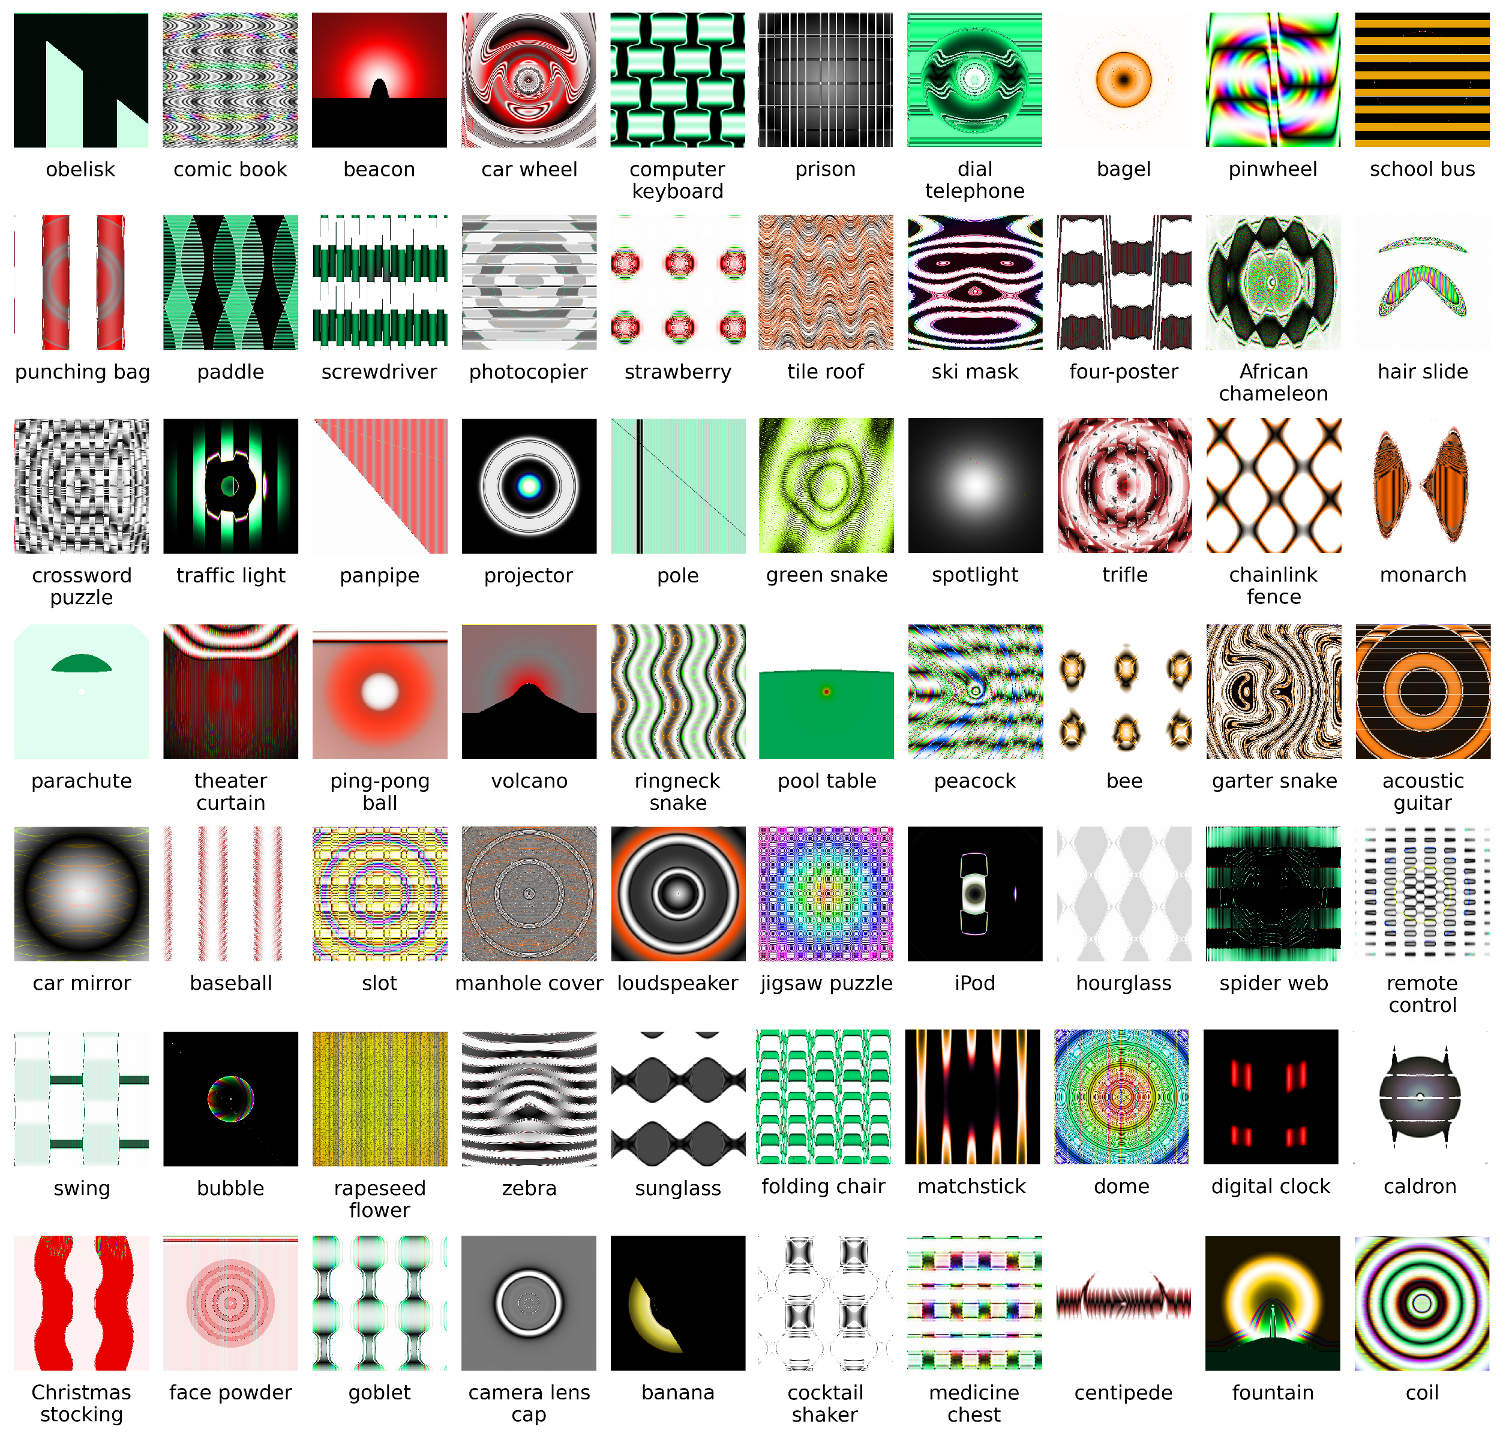
\includegraphics[width=1\textwidth]{fooled.jpg}
       	\label{fig:mesh20}
	 	 \caption{CNN got Fooled}
	\end{figure} 
 
 The neural network outputs its confidence in the image belonging to each of 1000 classes. The confidence scores across all 1000 classes must sum to 1, meaning that if one class is given 99.9\% confidence then the rest of the classes combined have less than 0.1\% confidence. In other words, in that case it is really declaring that it’s sure the image is of that class. It could also split its confidence between classes more evenly. For example, looking at a child climbing a tree it could give 60\% confidence to a “tree” class and 40\% confidence to a “child” class, but for most of the images shown above the network is certain the image belongs to one class. Humans are susceptible to optical illusions. Such illusions are designed to hack the way our brains see the world. Similarly, these images hack the way neural networks see the world. 
\subsection{Capsule neural networks}

Geoffrey E. Hinton’s new approach, known as capsule networks, is a twist on neural networks intended to make machines better able to understand the world through images or video. In one of the papers posted last month(November 2017), Hinton’s capsule networks matched the accuracy of the best previous techniques on a standard test of how well software can learn to recognize handwritten digits.

In the second paper, capsule networks almost halved the best previous error rate on a test that challenges software to recognize toys such as trucks and cars from different angles. Hinton has been working on his new technique with colleagues Sara Sabour and Nicholas Frosst at Google’s Toronto office.

Capsule networks aim to remedy a weakness of today’s machine-learning systems that limits their effectiveness. Image-recognition software in use today by Google and others needs a large number of example photos to learn to reliably recognize objects in all kinds of situations. That’s because the software isn’t very good at generalizing what it learns to new scenarios, for example understanding that an object is the same when seen from a new viewpoint.

To teach a computer to recognize a cat from many angles, for example, could require thousands of photos covering a variety of perspectives. Human children don’t need such explicit and extensive training to learn to recognize a household pet.

Capsules— small groups of crude virtual neurons—are designed to track different parts of an object, such as a cat’s nose and ears, and their relative positions in space. A network of many capsules can use that awareness to understand when a new scene is in fact a different view of something it has seen before.

Hinton formed his intuition that vision systems need such an inbuilt sense of geometry in 1979, when he was trying to figure out how humans use mental imagery. He first laid out a preliminary design for capsule networks in 2011. The fuller picture released last week was long anticipated by researchers in the field. 

\newpage
.%jhbhjb
\vspace{35mm}
\section*{\fontsize{14}{14}\selectfont Conclusion}

After the seminar, I was able to get a good idea about the recent trends in computer vision and also, I got an opportunity to share the knowledge with my friends and teachers during the seminar presentation.

Computer vision problems are yet to be solved. this is still a young and bright industry. The amount of visual data in this world is increasing in a massive rate and still researchers are trying to meaningfully arrange them and find some innovative technologies to make our lives better. 

Convolutional neural networks have been the buzz word for the last 4-5 years and it still has many possible applications in this world. Learning the basics of convolutional neural networks makes it easier for us to concentrate on many areas of Deep learning and also learn the new concepts such as Capsule Neural networks.

Overall, CapsNwt are the best way to do image classification now and it will remain the same for the next 1-2 years as other technologies are still under development stage.

\addcontentsline{toc}{section}{Conclusion}
\newpage
\section*{\fontsize{14}{14}\selectfont Referance}
\paragraph*{[1]}
A Study on Basics of Neural Network (Shaiqua Jabeen, Shobhana D. Patil, Shubhangi V. Bhosale, Bharati M. Chaudhari, Prafulla S. Patil) : nternational Journal of Innovative Research in Computer and Communication Engineering Vol.5,Issue 4, April 2017
\paragraph*{[2]}
Introduction to Neural Networks(R. Kruse et al., Computational Intelligence, Texts in Computer Science, DOI $10.1007/978-1-4471-7296-$3.2): Springer-Verlag London 2016
\paragraph*{[3]}
Recent Advances in Convolutional Neural Networks (Jiuxiang Gua, Zhenhua Wangb, Jason Kuenb, Lianyang Mab, Amir Shahroudyb, Bing Shuaib, Ting
Liub, Xingxing Wangb, Li Wangb, Gang Wangb, Jianfei Caic, Tsuhan Chenc):arXiv:1512.07108v6 [cs.CV] 19 Oct 2017
\paragraph*{[4]}
MobileNets: Efficient Convolutional Neural Networks for Mobile Vision Applications (Wei Liu, Dragomir Anguelov, Dumitru Erhan, Christian Szegedy, Scott Reed, Cheng-Yang Fu, Alexander C. Berg1): arXiv:1704.04861v1 [cs.CV] 17 Apr 2017
\paragraph*{[5]}
SSD: Single Shot MultiBox Detector (Wei Liu, Dragomir Anguelov, Dumitru Erhan, Christian Szegedy, Scott Reed, Cheng-Yang Fu1, Alexander C. Berg1):arXiv:1512.02325v5 [cs.CV] 29 Dec 2016
\paragraph*{[6]}
M. D. Zeiler, R. Fergus, Visualizing and understanding convolutional networks, in: Proceedings of the European Conference on Computer Vision (ECCV), 2014, pp. 818–833.
\paragraph*{[7]}
M. Rastegari, V. Ordonez, J. Redmon, A. Farhadi, Xnor-net: Imagenet classification using binary convolutional neural networks, in: Proceedings of the European Conference on Computer Vision (ECCV), 2016, pp. 525–542.]
\paragraph*{[8]}
Dynamic Routing Between Capsules( Geoffrey E. Hinton, Google Brain Toronto with Sara Sabour, Nicholas Frosst {sasabour, frosst, geoffhinton}@google.com)) arXiv:1710.09829v1 [cs.CV] 26 Oct 2017
\paragraph*{[9]}
\label{figmesh9} Fast R-CNN(Ross Girshick
Microsoft Research): arXiv:1504.08083v2 [cs.CV] 27 Sep 2015
\paragraph*{[10]} R-FCN: Object Detection via Region-based Fully Convolutional Networks(Jifeng Dai(Microsoft Research) ,Yi Li( Tsinghua University),
,Kaiming He(Microsoft Research)
Jian Sun(
Microsoft Research)):arXiv:1605.06409v2 [cs.CV] 21 Jun 2016
\paragraph{[11]} Applications of Convolutional Neural Networks (Ashwin Bhandare
, Maithili Bhide
, Pranav Gokhale
, Rohan Chandavarkar
):(IJCSIT) International Journal of Computer Science and Information Technologies, Vol. 7 (5) , 2016, 2206-2215

\paragraph{[12]} Deep Residual Learning for Image Recognition(Kaiming He, Xiangyu Zhang, Shaoqing Ren, Jian Sun):arXiv:1512.03385v1 [cs.CV] 10 Dec 2015

\paragraph{[13]}MobileNets: Efficient Convolutional Neural Networks for Mobile Vision Applications (Andrew G. Howard, Menglong Zhu, Bo Chen, 
Dmitry Kalenichenko, Weijun Wang, 
Tobias Weyand, Marco Andreetto,  
Hartwig Adam):arXiv:1704.04861v1 [cs.CV] 17 Apr 2017

\paragraph{[14]}nception-v4, Inception-ResNet and
the Impact of Residual Connections on Learning (Christian Szegedy, Sergey Ioffe, Vincent Vanhoucke ):arXiv:1602.07261v2 [cs.CV] 23 Aug 2016

\paragraph{[15]}Going deeper with convolutions(Christian Szegedy, Wei Liu, Yangqing Jia, Pierre Sermanet, Scott Reed, Dragomir Anguelov, Dumitru Erhan, Vincent Vanhoucke, Andrew Rabinovich):arXiv\footnote{arXiv.org (Cornell Univercity Library) :arXiv is an e-print service in the fields of physics, mathematics, computer science, quantitative biology, quantitative finance, statistics, electrical engineering and systems science, and economics. Submissions to arXiv should conform to Cornell University academic standards. arXiv is owned and operated by Cornell University, a private not-for-profit educational institution. arXiv is funded by Cornell University Library, the Simons Foundation and by the member institutions.}:1409.4842v1 [cs.CV] 17 Sep 2014

\paragraph{[16]}Deep Neural Networks are Easily Fooled:
High Confidence Predictions for Unrecognizable Images(Anh Nguyen, Jason Yosinski, Jeff Clune):Computer Vision and Pattern Recognition (CVPR ’15), IEEE, 2015.



\addcontentsline{toc}{section}{Referance}
\end{document}
 
